\chapter{Feature Extraction}
Image stitching process starts  from feature extraction. In previous chapter, I introduced the basics of corner detection in an image. Each corner in an image has features and we try extract the corners in images and assign features to them. There are some notable advantages using corners as features:
\begin{enumerate}
	\item Instead of matching all the pixels in an image, we focus on matching corners only. Since the number of corners is much smaller than the total number of pixels, matching is faster.
	\item Since corner is a point, it is easy to get transformation parameters using the locations of the matching corners. 
\end{enumerate}
Like every image processing task, the feature extraction starts with preprocessing (section~\ref{sec:preprocessing}) to remove image noise, correct intensity differences etc. There are several algorithms for feature extraction, I have discussed the most popular feature extraction methods (i.e. Harris, SIFT, SURF) in section~\ref{sec:feature-extraction}.

\section{Preprocessing}
\label{sec:preprocessing}
This section discusses some preprocessing techniques before we actually carry out the stitching. The X-ray images might not be perfect for stitching; the noise present in the image cause inaccurate stitching, the high resolution images are slower or sometimes the intensity different between the images gives unpleasant stitched result. The X-ray images should be preprocessed before they are input for feature extraction. For image stitching problem, we generally focus on the following preprocessing steps:
\begin{description}
	\item [Noise Reduction] The noise in the image gives inaccurate result; so noise reduction is a crucial step in stitching. There are several smoothing operators (see section~\ref{sec:image-smoothing}) which can be implemented to suppress the noise in the image. The smoothing should not reduce the image information that we use for stitching. So, experimentally decide the effective image smoother and its parameters.
	
	\item [Intensity Leveling] To get the better stitching result, the images to be stitched should have similar intensity. The intensity differences in the images actually effects the key points identification process because the same image with different intensities result different key points. Similarly, we have to implement more effective blending operations because different intensity images generate a visible seam in the join of images. So, intensity leveling technique makes the image intensities similar to get better stitching result. 
	\item [Overlapping Area Prediction \& Selection] Sometimes, if we already know some information regarding alignment, we can use this information to simplify the image stitching task. For X-ray images, images are always either aligned vertically or horizontally. So, if images are aligned horizontally, we can predict that the second half of the first image and first half of the second image have high probability of overlapping. We select the second half of first image and first half of the second image for faster estimation of motion parameters. 
\begin{figure}%
\centering
\subfloat[]{%

\includegraphics[scale=0.15]{2.mainmatter/2.Methodology/figures/left}
\label{fig:left}%
}
\qquad
\subfloat[]{%
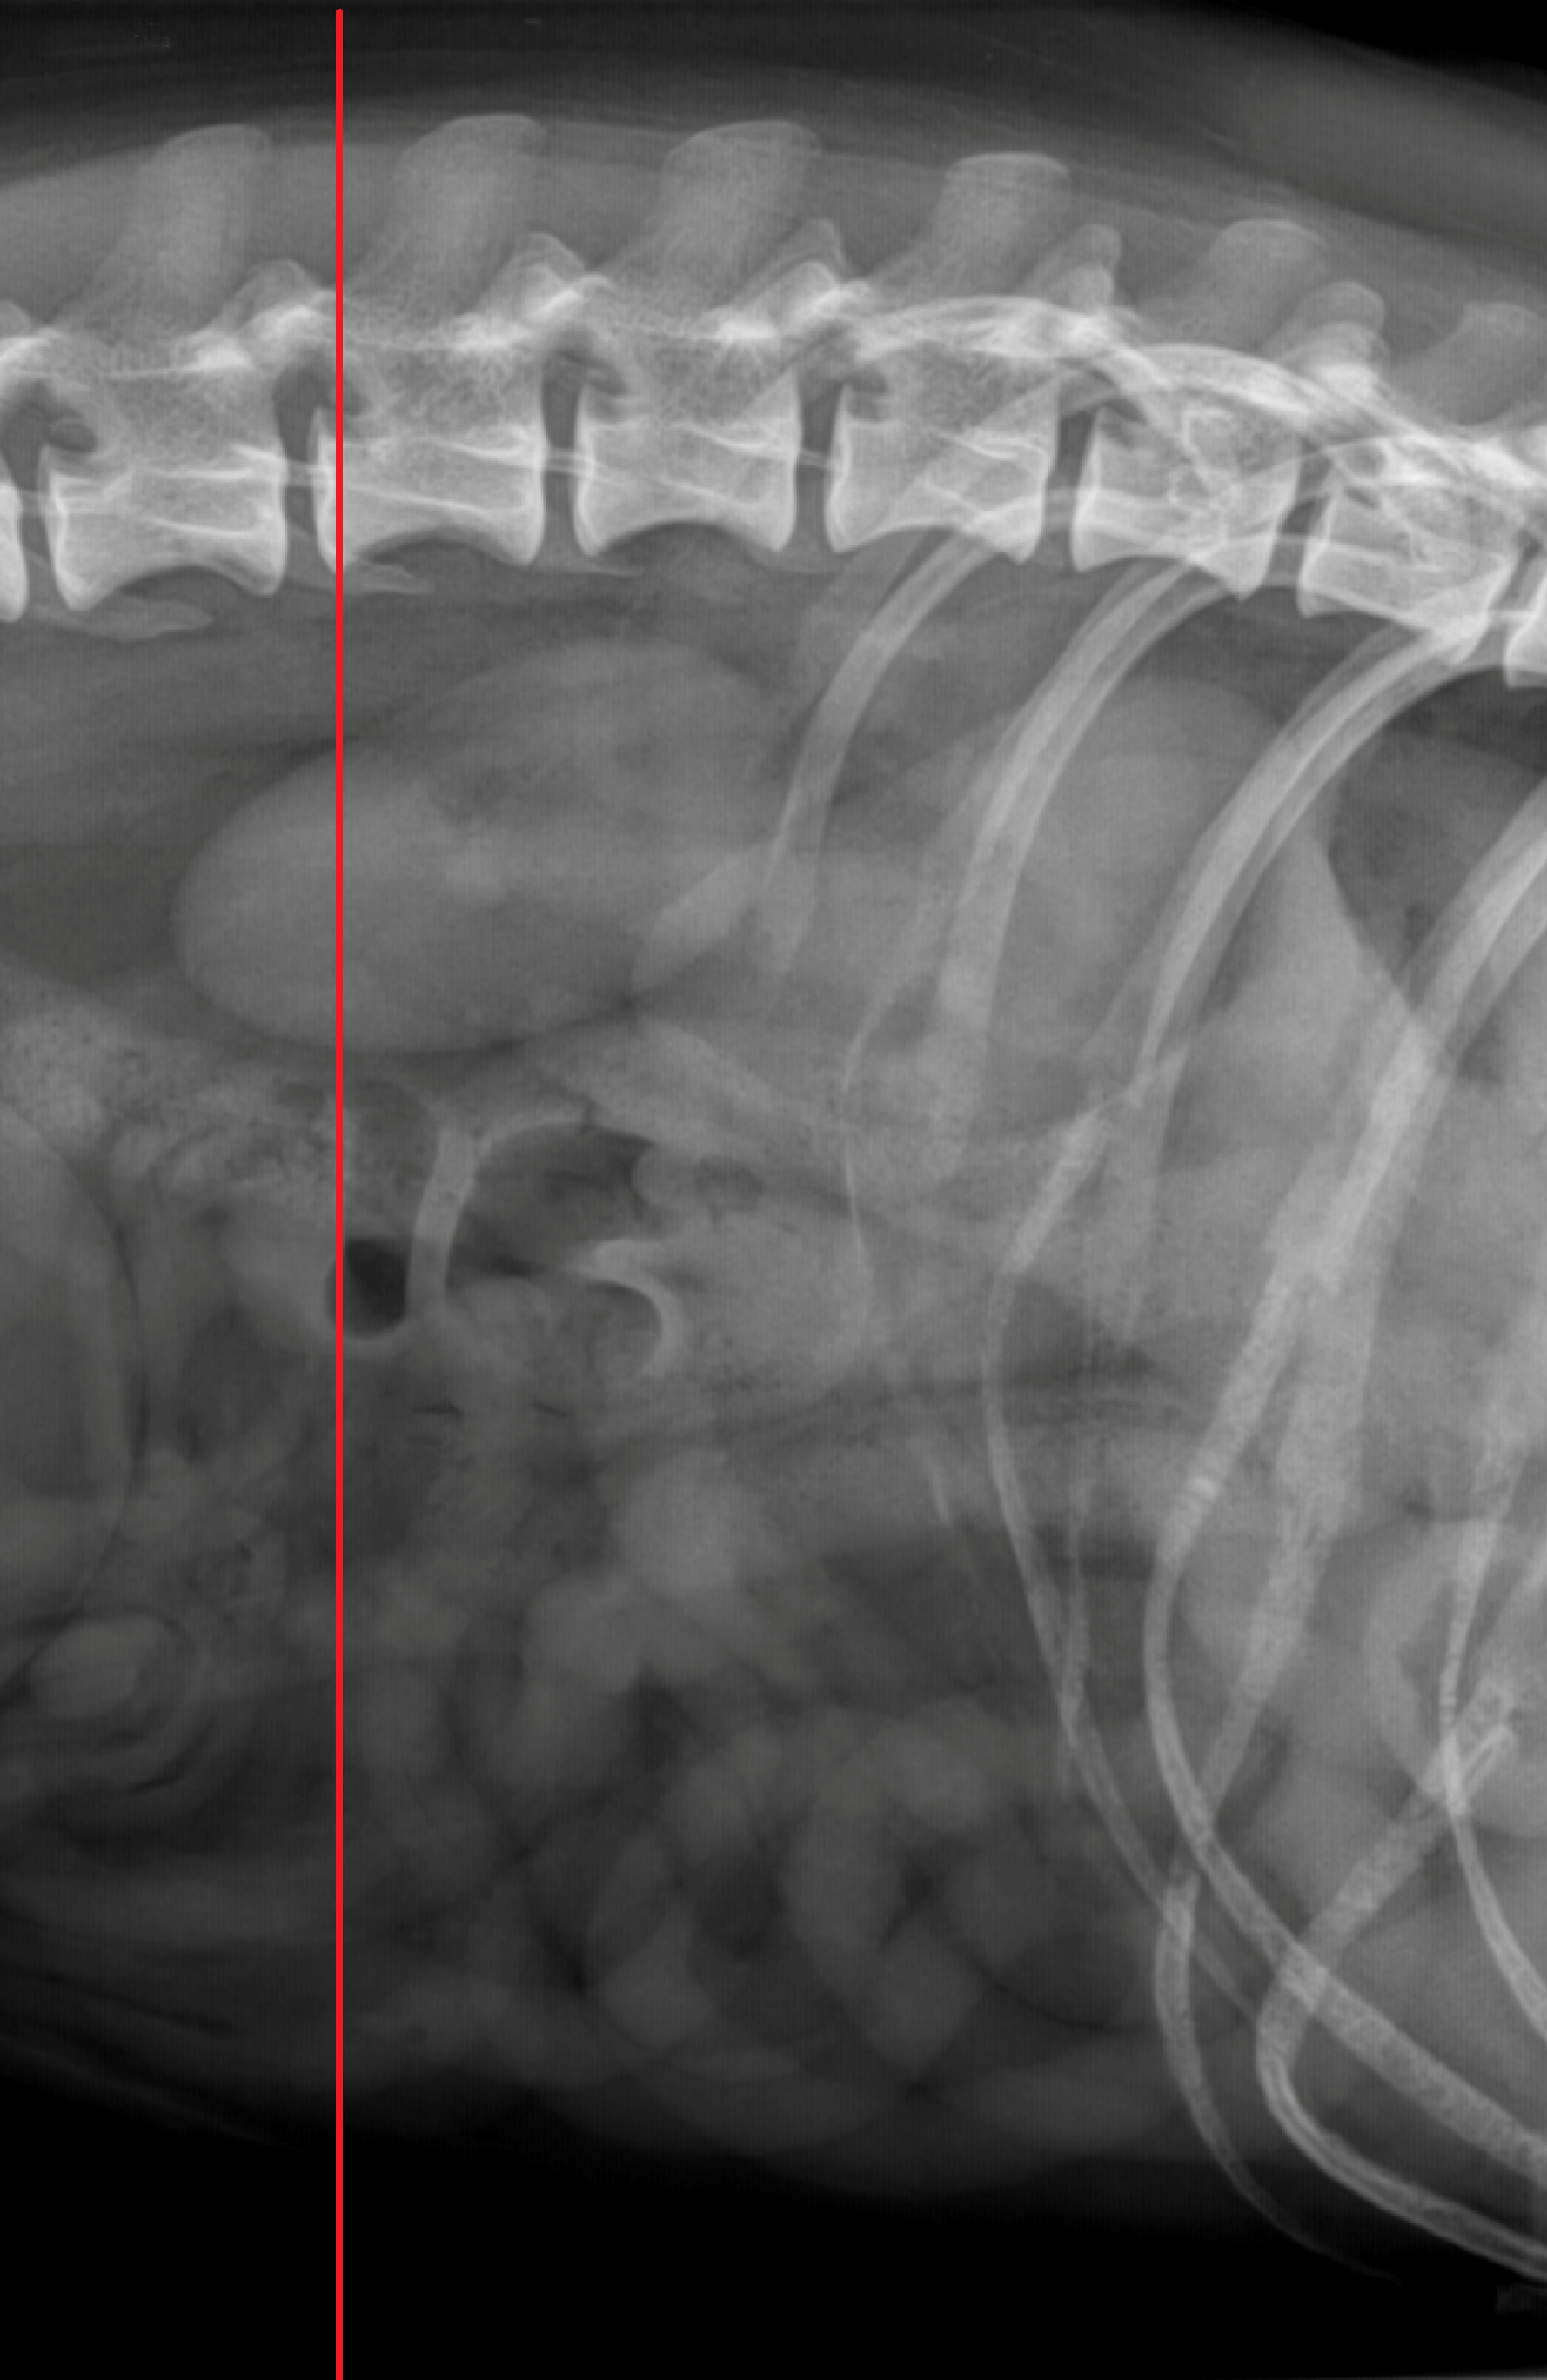
\includegraphics[scale=0.15]{2.mainmatter/2.Methodology/figures/right}%
\label{fig:right}%
}%
\caption[Overlapping Area Prediction]{The second half of figure~\subref{fig:left} and the first half of figure~\subref{fig:right} chosen for faster estimation of motion parameters. The vertical line separates the overlapped region.}%
\label{fig:overlap-estimation}%
\end{figure}	
\end{description}

%Intensity levelling
%Noise Reduction
%Cropping Unnecessary Parts

\section{Feature Extraction}
\label{sec:feature-extraction}
% Description of Harris Corner Detector
% Problems with Harris Corner Detection
% Alternative of Harris (SIFT or SURF)
% Comparison of SIFT & SURF
% Description of why SURF is better than SIFT
% Feature matching Methods: Distance Measure(K-nn)
% 
There are several corner detection algorithms. In this section, I will describe \emph{Harris Corner Detector}, and modern corner detectors such as \emph{Scale Invariant Feature Transform (SIFT)} \& \emph{Speeded UP Robust Feature (SURF)}:

\subsection{Harris Corner Detection}
\label{subsec:harris-corner-detection}
The Harris Corner Detection was developed by \emph{Chris Harris} and \emph{Mike Stephens} in 1988~\cite{Parks:11}. It is widely used algorithms for corner detection.\\

\noindent The Harris algorithm can be described as follows~\cite{Parks:11}:\\

\noindent \textbf{Input:}\textit{Gray-scale Image, Gaussian Variance (radius of window=3 x standard deviation),k value, threshold T}\\
\textbf{Output:}\textit{Map with position of detected corners}\\
\begin{enumerate}
	\item For each pixel $(x,y)$ in the image, calculate the \emph{auto correlation matrix} $M$ as follows:\\ 
	\begin{equation}
		M=\left[ \begin{array}{cc}
			A & C\\
			C & B 
		\end{array}
		\right] 
	\label{eq:hessian-matrix}
	\end{equation}			
	where 
	\begin{equation}
					A=\left(\frac{\partial I}{\partial x}\right)^2 \otimes w 
	\label{eq:A}
	\end{equation}
	
	\begin{equation}
	        B=\left( \frac{\partial I}{\partial y} \right)^2 \otimes w, 
	\label{eq:B}
	\end{equation}
	
	\begin{equation}
				 C=\left( \begin{array}{c}\frac{\partial I}{\partial x} \frac{\partial I}{\partial y}\end{array}\right) \otimes w
	\label{eq:C}
	\end{equation} 
				$\otimes$ is the convolution operator\\
				and, $w$ is the Gaussian window	
						
\item Construct the \emph{cornerness map} by calculating the cornerness measure $Cornerness(x,y)$ for each pixel (x,y):\\
\begin{equation}
Cornerness(x,y)=det(M)-k(trace(M))^2
\label{eq:cornerness-map}
\end{equation} 
where 
\begin{equation}
det(M)=AB-C^2 \approx \lambda_1 \lambda_2,
\label{eq:deter-M}
\end{equation}

\begin{equation}
trace(M)=A+B \approx \lambda_1+ \lambda_2
\label{eq:trace-M}
\end{equation}
and\\
k=a constant (generally, k between 0.04 to 0.5 gives good result.)

\item Threshold the interest map by setting all $Cornerness(x,y)$ below a threshold $T$ to zero. The number of corners depends upon the selected threshold $T$, decreasing $T$ results increment in corners.
\item Perform non-maximal suppression to find local maxima.
 The non-zero points remaining in the cornersness map are corners.					
	 
\end{enumerate}

\subsection{SIFT}
\label{subsec:SIFT}
The simple corner detectors like Harris (section~\ref{subsec:harris-corner-detection}) can work only when the images are similar in  nature (same scale, orientation, intensity etc)~\cite{Lowe:04}. The SIFT features are invariant to image scaling and rotation, and partially invariant to change in illumination and 3D camera viewpoint. The features are highly distinctive ensuring a single feature to be correctly matched with high probability against a large database of features, thus making it applicable to image registration~\cite{Lowe:04}. \\ 

\noindent SIFT features detection consists of following steps:
\begin{enumerate}
	\item \textbf{Scale-space extrema detection:} This step finds out the potential interest points which are invariant to scale and orientation. This is carried out by using a difference of Gaussian (DoG) function. Extreme points are searched over all scales and image locations. The \emph{Difference of Gaussian} function is convolved with the image to get DoG image $D(x,y,\sigma)$. Mathematically, this can be represented as follows: 

\begin{equation}
D(x,y,\sigma)=(G(x,y,k \sigma)-G(x,y,\sigma))*I(x,y) 
\label{eq:state-space-image}
\end{equation}
which is equivalent to 
\begin{equation}
D(x,y,\sigma)=L(x,y,k \sigma)-L(x,y, \sigma)
\label{eq:equiv-state-space}
\end{equation}
where $G(x,y,\sigma)$ is Gaussian function [equation~\ref{eq:gaussian-function}]. $k$ is constant multiplicative factor. The \emph{DoG} function is preferred to \emph{Laplacian of Gaussian (LoG)} because it is simple to compute and the result can be close approximation to LoG~\cite{Lowe:04}. David Lowe has derived the relationship of LoG and DoG images as:

\begin{equation}
G(x,y,k \sigma)-G(x,y, \sigma) \approx (k-1)\sigma^2 \Delta^2G
\label{eq:dog-log}
\end{equation}
which shows DoG and LoG are differed only by a constant factor $k-1$. \\

\noindent This stage consists of two processes:\\
\textit{Construction of DoG images} As shown in figure~\ref{fig:dog-const}, the initial image is incrementally convolved with Gaussians to produce images separated by a constant factor $k$ in scale space (the left column in the figure). The approximation error will be zero when $k$ is 1 and David Lowe in~\cite{Lowe:04} also claims the stability of extrema even with significant differences in scale even when $k=\sqrt{2}$. For each octave of scale space (doubling of $\sigma$),the top image is re-sampled by taking every second pixel in each row and column to create the initial image for next octave with double $\sigma$ which greatly simplifies the computation. The adjacent images in the stack of the octave are subtracted to produce the DoG images as shown in figure~\ref{fig:dog-const}.\\

\begin{figure}[H]%
\centering
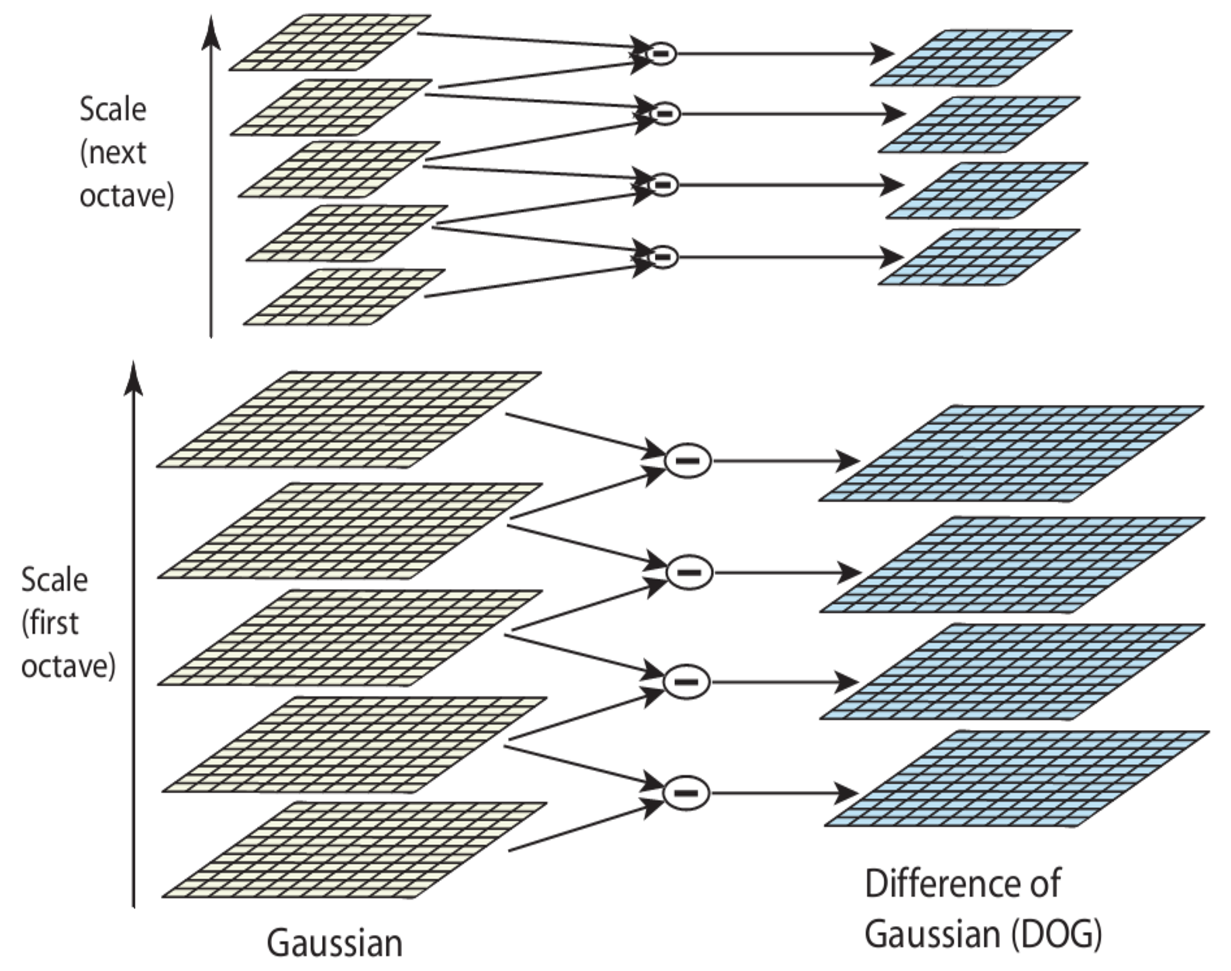
\includegraphics[width=0.9\columnwidth]{2.mainmatter/2.Methodology/FeaturesExtraction/figures/SIFT/difference-of-gaussian}%
\caption[Construction of DoG Image]{Construction of DoG image. \imgsrc{(Image source: Lowe~\cite{Lowe:04})}}%
\label{fig:dog-const}%
\end{figure}

\textit{Local extrema detection} As shown in figure~\ref{fig:max-min-dog}, the local maxima and minima of DoG images are found out by comparing each sample point to its eight neighbors in the current image and nine neighbors in the scale above and below. In 2D situation, we need to compare 3 DoG images in each octave, so we have to construct 4 different scale images~\cite{Li:11}.

\begin{figure}%
\centering
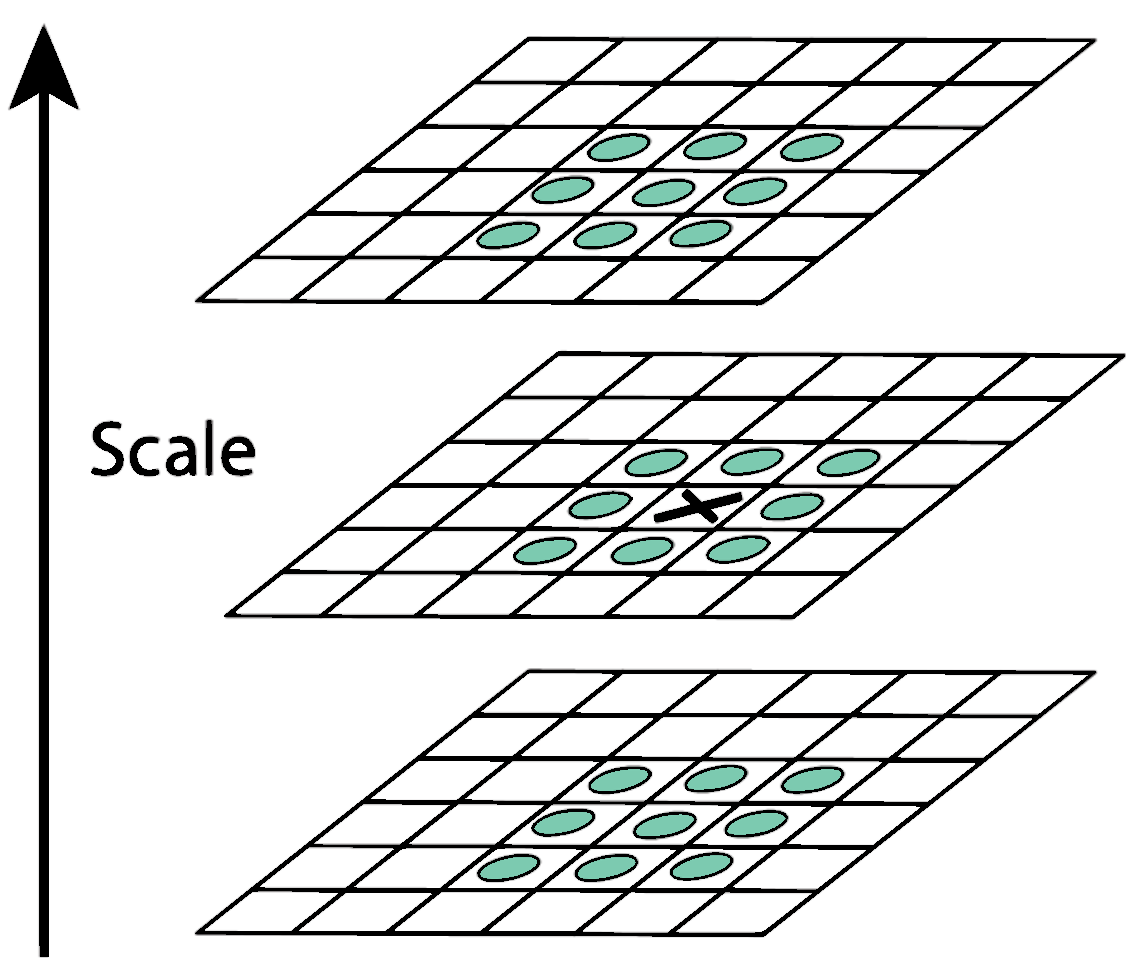
\includegraphics[width=0.6\columnwidth]{2.mainmatter/2.Methodology/FeaturesExtraction/figures/SIFT/maxima-minima-identification}%
\caption[Maxima and Minima of DoG Images]{Maxima and minima idenfication of DoG images. \imgsrc{(Image Source: Lowe~\cite{Lowe:04})}}%
\label{fig:max-min-dog}%
\end{figure}

\item \textbf{Key point localization:} This step performs a detailed fit to nearby data for location, scale, and ratio of principal curvatures so that we can remove the points with low contrast or poorly localized along the edge.\cite{Lowe:04}. To remove low contrast points, the magnitude of intensity is compared with a certain value, if it is less than the value, then reject it. Brown~\cite{Brown:02} suggested to use \emph{Taylor expansion} of the value at the extreme points to get the intensity. Similarly, to remove the edges, we use principal of Harris Corner Detector (section~\ref{subsec:harris-corner-detection}) i.e. in any point, if the ratio of largest magnitude eigenvalue and the smaller one is greater than some threshold, then it indicates the edge point. Suppose, $r$ is the threshold ratio of the two principal eigenvalues and $M$ is auto correlation matrix, we check the condition (modification of equation~\ref{eq:cornerness-map}):  
\begin{equation}
\frac{trace(M)^2}{det(M)}<\frac{(r+1)^2}{r}
\label{eq:edge-check}
\end{equation}

\item \textbf{Orientation assignment:} The orientation is assigned as key point descriptor so that we can achieve invariance to image rotation~\cite{Lowe:04}. Lowe suggests to use the following method for each key point to have stable results. The magnitude, $m(x,y)$ and orientation, $\theta(x,y)$  of the gradient is computed as:
\begin{equation}
m(x,y)=\sqrt{(L(x+1,y)-L(x-1,y))^2+(L(x,y+1)-L(x,y-1))^2}
\label{eq:orient-mag}
\end{equation}

\begin{equation}
\theta(x,y)=\tan^{-1}\frac{L(x,y+1)-L(x,y-1)}{L(x+1,y)-L(x-1,y)}
\label{eq:orient-theta}
\end{equation}
Lowe suggests to form an \emph{orientation histogram} from the gradient orientations of sample points withing a region around a key point and detect the highest peak. Any other local peak that is within 80\% of the highest peak is used to also create a key point with that orientation. So, for locations with multiple peaks of similar magnitude, there will be multiple key points created at the same location and scale but with different orientations~\cite{Lowe:04}.

\item \textbf{Keypoint descriptor}
In above steps, we defined the image location, scale, orientation of each key point. In this step, we compute a descriptor which is highly distinctive for each key point while being invariant to change in illumination or 3D viewpoint. This can be achieved by selecting a window around the key point and generating the feature vectors. Suppose we selected 16x16 window, then we break it into 4x4 windows as shown in figure~\ref{fig:keypoint-descriptor}. For each window, we calculate the gradient magnitude and orientation at each point. Again, the magnitude is weighted according to the distance from key point (use Gaussian weighting function~\cite{Lowe:04}), i.e. gradients that are far away from the key point will add smaller values. A 8 bin orientation histogram thus carries 8 features for each small window. Thus for 16x16 window, we can have a feature vector of the key point with 16x8=128 features in it which uniquely describes the key point.

\begin{figure}%
\centering
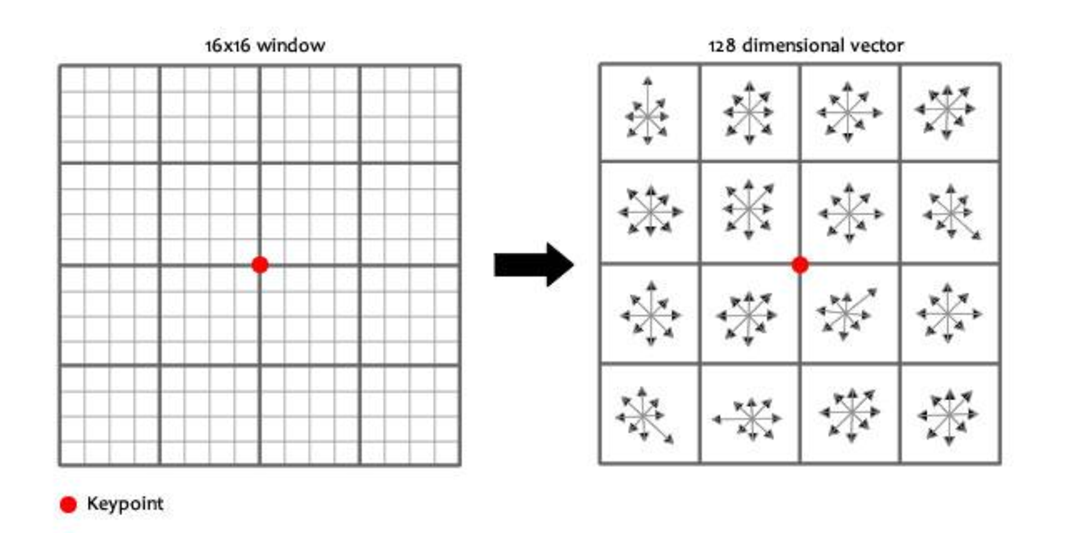
\includegraphics[width=0.9\columnwidth]{2.mainmatter/2.Methodology/FeaturesExtraction/figures/SIFT/keypoint-descriptor}%
\caption[Creation of Key-point Descriptor]{Creation of keypoint descriptor. Image gradients are used to create image descriptor. \imgsrc{(Image source: Sinha~\cite{Sinha:10:online})}}%
\label{fig:keypoint-descriptor}%
\end{figure}
\end{enumerate}

\subsection{SURF}
\label{subsec:SURF}
The dimension of the descriptor has a direct impact on the time it takes and less dimensions are desirable for fast interest point matching~\cite{Bay:08}. SIFT has 128 dimensional feature vector, which makes it very slow making it not suitable for real time applications. the high dimensionality of the descriptor is a drawback of SIFT at matching step. For online applications replying only on regular PC, each one of the three steps (detection, description, matching) has to be fast. Therefore, SURF method of feature detection has been developed to overcome the drawback of SIFT i.e. making matching algorithm faster by creation of low dimensional feature vector. \\

\noindent The SURF method can be described by the following two steps:\\
\begin{enumerate}
	\item \textbf{Interest Point Detection}
	\begin{itemize}
	    \item {\textit{Integral Images}} The computation time is reduced drastically by  using an intermediate representation of the image called \emph{integral image}~\cite{Viola:01}. The value at a location \textbf{X}=$(x,y)^T$ of integral image $II(\textbf{X})$ is calculated as:
	\begin{equation}
	II(\textbf{X})=\sum_{i=0}^{i \leq x}{\sum_{j=0}^{j\leq y}{I(i,j)}}
	\label{eq:integral-image}
	\end{equation}
	After computing of integral image, we can calculate the intensity of any vertical rectangle as shown in figure~\ref{fig:intensity-calculation}. The calculation time is independent of the the size.
	
	\begin{figure}[H]%
	\centering
	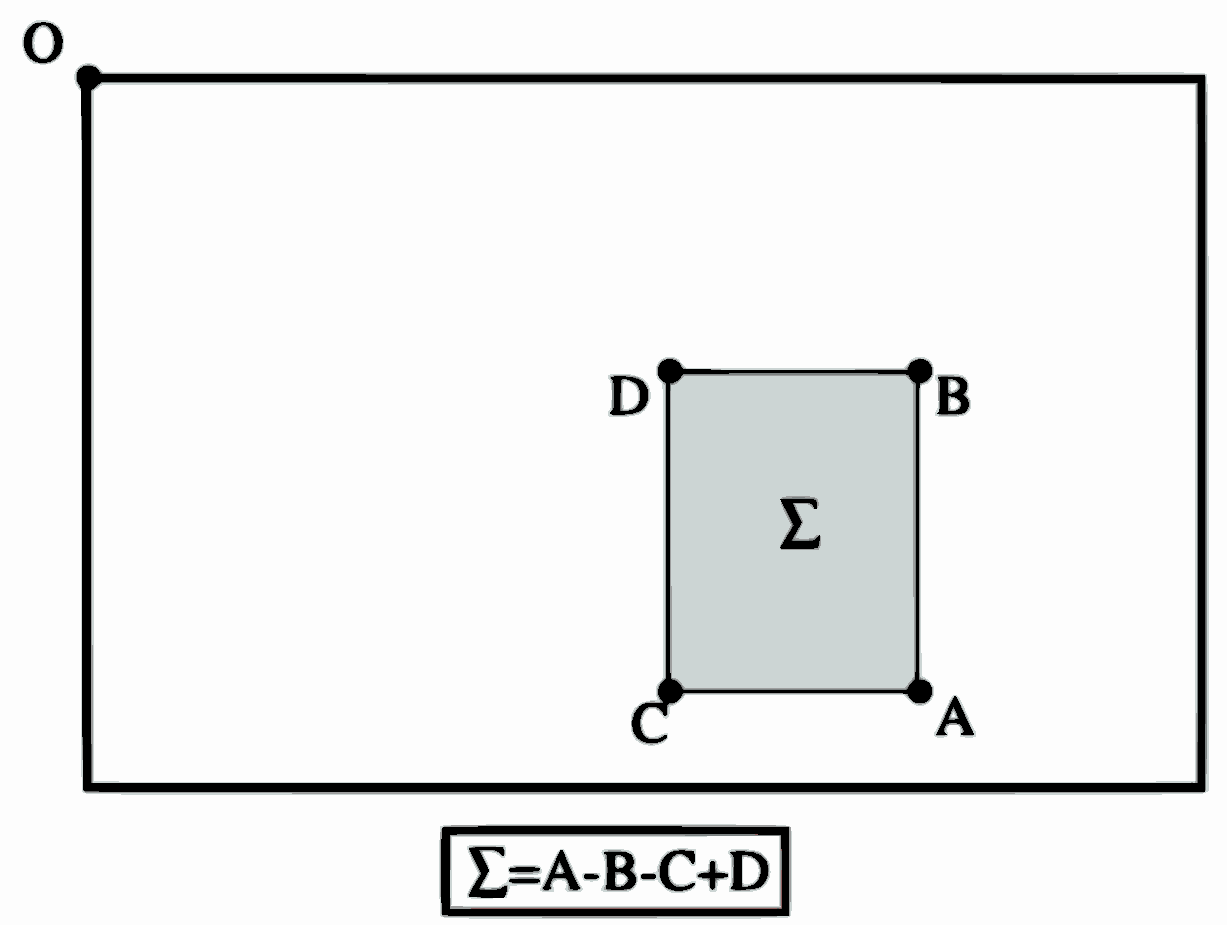
\includegraphics[width=0.6\columnwidth]{2.mainmatter/2.Methodology/FeaturesExtraction/figures/SURF/intensity-calculation}%
	\caption[Calculation of Sum of Intensities]{Calculation of sum of intensities inside a rectangular region of integral image. \imgsrc{(Image source: Bay \emph{et al}~\cite{Bay:08})}}%
	\label{fig:intensity-calculation}%
	\end{figure}
	\item {\textit{Hessian matrix}} For any point \textbf{x} = (x,y) in image $I$, the Hessian matrix $H(x,\sigma)$ can be defined as:\\
	\begin{equation}
  H(x,\sigma)=\left[ \begin{array}{cc}
	L_{xx}(x,\sigma) & L_{xy}(x,\sigma)\\
	L_{xy}(x,\sigma) & L_{yy}(x,\sigma)	
\end{array}
\right]
\label{eq:hess-matrix}
\end{equation}
where
\begin{equation} L_{xx}(x,\sigma)=\frac{\partial^2}{\partial_x^2}g(\sigma)\otimes I
\label{eq:Lxx}
\end{equation}

\begin{equation}
L_{yy}(x,\sigma)=\frac{\partial^2}{\partial_y^2}g(\sigma)\otimes I
\label{eq:Lyy}
\end{equation}


\begin{equation}
L_{xy}(x,\sigma)= \frac{\partial^2}{\partial_x \partial_y}g(\sigma) \otimes I
\label{eq:Lxy}
\end{equation}
The Gaussian functions are discretized and cropped, so there is some loss of repeatability of Hessian based detectors under image rotations; but this is out-weighted by the advantage of fast convolution by the descretization and cropping~\cite{Bay:08}. The approximated determinant of Hessian matrix represents the blob response in the image at location \textbf{x}. Bay \emph{et al.}\cite{Bay:08} suggests to use 9x9 box filters as shown in figure~\ref{fig:approx-gaussian-partial} to create the blob responses $D_{xx}$, $D_{yy}$, $D_{xy}$. Then computation of determinant of Hessian i.e. $det(H_{approx})$ is computed as follows:
\begin{equation}
det(H_{approx})=D_{xx}D_{yy}-w(D_{xy}^2)
\label{eq:det-hessian-apprx}
\end{equation}
here, w is used to balance the expression for the Hessian's determinant. Generally, it does not have a significant impact on the result, so we keep this value as constant\cite{Bay:08}. \\

\begin{figure}[H]%
\centering
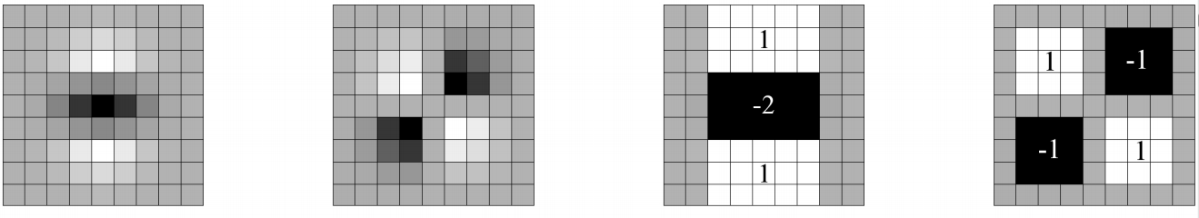
\includegraphics[width=\columnwidth]{2.mainmatter/2.Methodology/FeaturesExtraction/figures/SURF/approx-gaussian-partial}%
\caption[Approximation of Gaussian Partial Derivative]{Left two images are cropped and decretized Gaussian second order partial derivative ($L_{yy}$, $L_{xy}$), right two images are corresponding approximated filters ($D_{yy}$, $D_{xy}$).}%
\label{fig:approx-gaussian-partial}%
\end{figure}
\item{\textit{Scale Space Representation}}
\noindent The scale space is analyzed by up-scaling the box filter size rather than iteratively reducing the image size (figure~\ref{fig:upscaling}). The output of the 9 x 9 filter is the initial scale layer (scale=1.2, because the approximation was with $\sigma$=1.2). By doing this, we achieve computational efficiency and there will be no aliasing because we don't need to down-sample the image~\cite{Bay:08}.\\


\begin{figure}%
\centering
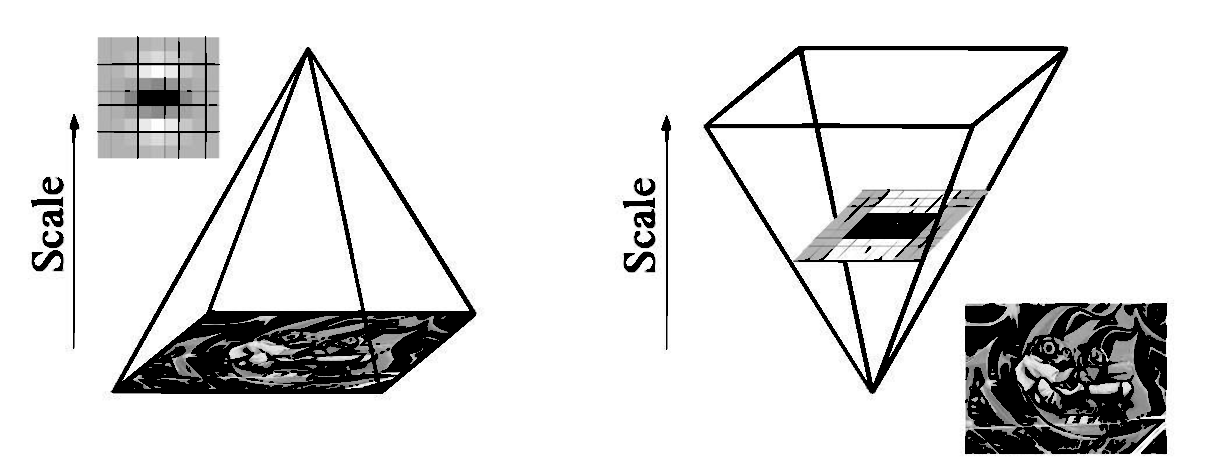
\includegraphics[width=\columnwidth]{2.mainmatter/2.Methodology/FeaturesExtraction/figures/SURF/upscaling-integral}%
\caption[Scale Space Generation]{The use of integral images allows up-scaling of the filter at constant cost.}%
\label{fig:upscaling}%
\end{figure}

\noindent The scale space is divide into octaves. An octave represents a series of filter response maps obtained by convolving the same input image with a filter of increasing size. Each octave is divided into a constant number of scale levels as shown in figure~\ref{fig:filters-octaves}

\begin{figure}[H]%
\centering
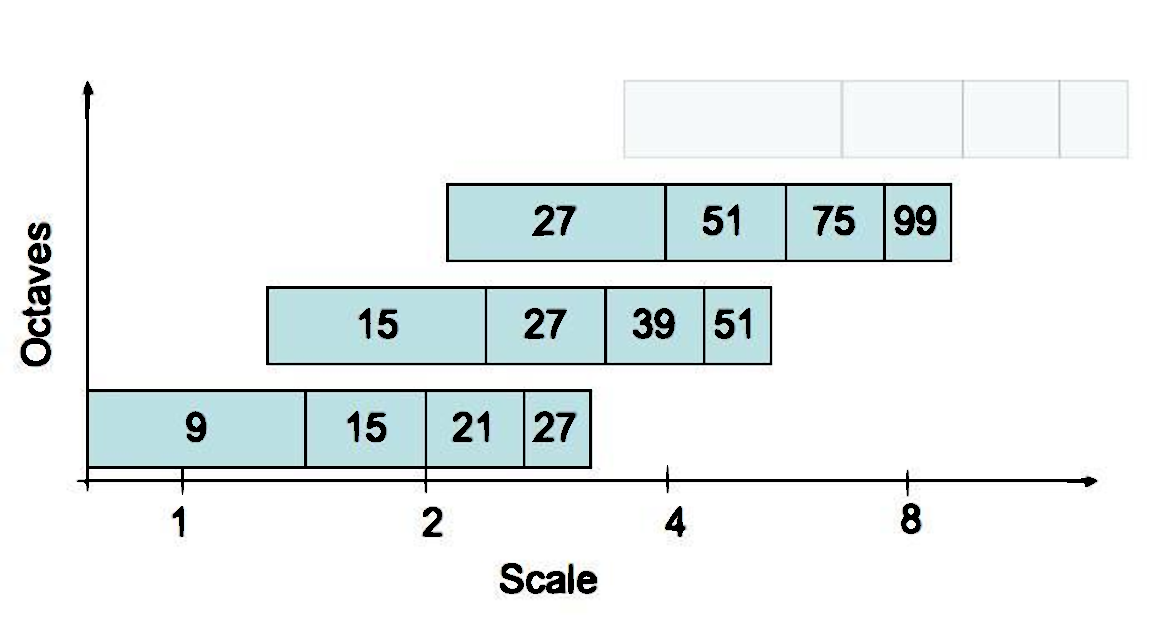
\includegraphics[width=0.6\columnwidth]{2.mainmatter/2.Methodology/FeaturesExtraction/figures/SURF/octaves-scales}%
\caption[Scaling in Octaves]{Filter side lengths for three different octaves. \imgsrc{(Image source: Bay \emph{et al}~\cite{Bay:08})}}%
\label{fig:filters-octaves}%
\end{figure}

\item {\textit{Interest Point Localization}}
After successful, scale-space creation, the next task is to localize the interest points.To localize interest points in the image and over scales, a non-maximum suppression in a 3 x 3 x 3 neighborhood is applied. The maxima of the determinant of the Hessian matrix are then interpolated in scale and image space.\cite{Bay:08}.
\end{itemize} 
	
\item \textbf{Interest Point Description} The method of descriptor extraction is similar to SIFT described in previous section. The distribution of first order Haar wavelet responses in x and y direction (figure~\ref{fig:haar-wavelets}) instead of the gradient is used for descriptor extraction. We exploit integral images for speed. The use of only 64 dimensional feature vector greatly reduces the time for matching while increasing the robustness~\cite{Bay:08}. The authors of SURF claims the new indexing step based on the sign of the Laplacian increases the robustness of the descriptor and matching speed also; so the name SURF-Speeded-Up Robust Features.\\

\begin{figure}[H]%
\centering

\includegraphics[width=\columnwidth]{2.mainmatter/2.Methodology/FeaturesExtraction/figures/SURF/haar-wavelets}%
\caption[Haar Wavelets]{Haar Wavelets: The left one is response in x-direction, the right one is response in y-direction. Weight=1 for black region, -1 for white region. \imgsrc{(Image source: Evans~\cite{Evans:09})}}%
\label{fig:haar-wavelets}%
\end{figure}


The interest points descriptors are assigned by the following two steps:
\begin{itemize}
	\item {\textit{Orientation Assignment}} Orientation assignment is carried out for rotation invariance. Haar wavelet responses of size 4$\sigma$ are calculated for a set of pixels within a radius of 6$\sigma$ of detected point.\footnote{$\sigma$ is the scale at which the point was detected.} The specific set of pixels is determined by sampling those from within the circle using step size of $\sigma$~\cite{Evans:09}. Weighted responses with a Gaussian centered at the interest point are used to find the dominant orientation in each circle segment of angle $\frac{\pi}{3}$ (i.e. 60\deg) around the origin. At each position, the x and y- responses within the segment are summed and used to form a new vector. The longest vector is the orientation of the interest point~\cite{Evans:09}.This process is shown in figure~\ref{fig:orientation-assignment}.
	
	
	\begin{figure}[H]%
	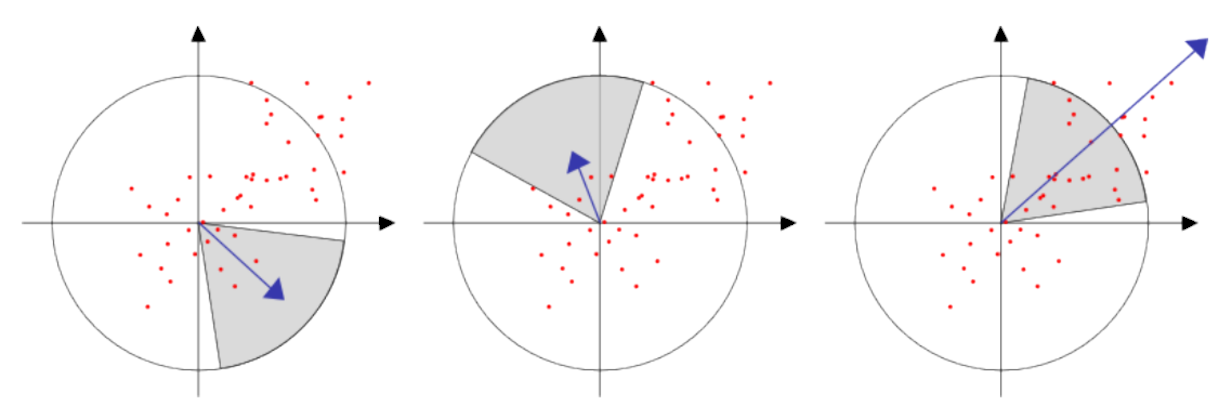
\includegraphics[width=\columnwidth]{2.mainmatter/2.Methodology/FeaturesExtraction/figures/SURF/orientation-assignment}%
	\caption[Orientation Assignment]{Orientation Assignment: The blue arrow is the sum of the responses. The largest one determines the dominant orientation. \imgsrc{(Image source: Evans~\cite{Evans:09})}}%
	\label{fig:orientation-assignment}%
	\end{figure}	
	
	\item{\textit{Descriptor Components}} We construct a square window of size 20$\sigma$ around the interest point. The orientation of the window will be the dominant orientation we calculated above. This descriptor window is divided into 4 x 4 regular sub-regions. We select 25 regularly distributed sample points in each sub-region and Haar wavelets of size 2$\sigma$ are calculated for those points~\cite{Evans:09}. Then, the feature vector for each sub-region will be
	\begin{equation}
	V_{subregion}=\left[ \Sigma dx,\Sigma dy,\Sigma \left| dx \right|,\Sigma \left| dy\right| \right]
	\label{eq:feature-vector}
	\end{equation}
	
	
As shown in figure~\ref{fig:descriptor-components}, each sub-region will have four values to the descriptor vector which results the overall vector length 4 x 4 x 4=64. Evans in his article~\cite{Evans:09} claims that the result SURF descriptor is invariant to rotation, scale, brightness and contrast\footnote{invariant to contrast is achieved after reduction to unit length~\cite{Evans:09}.}.
\begin{figure}[H]%
	   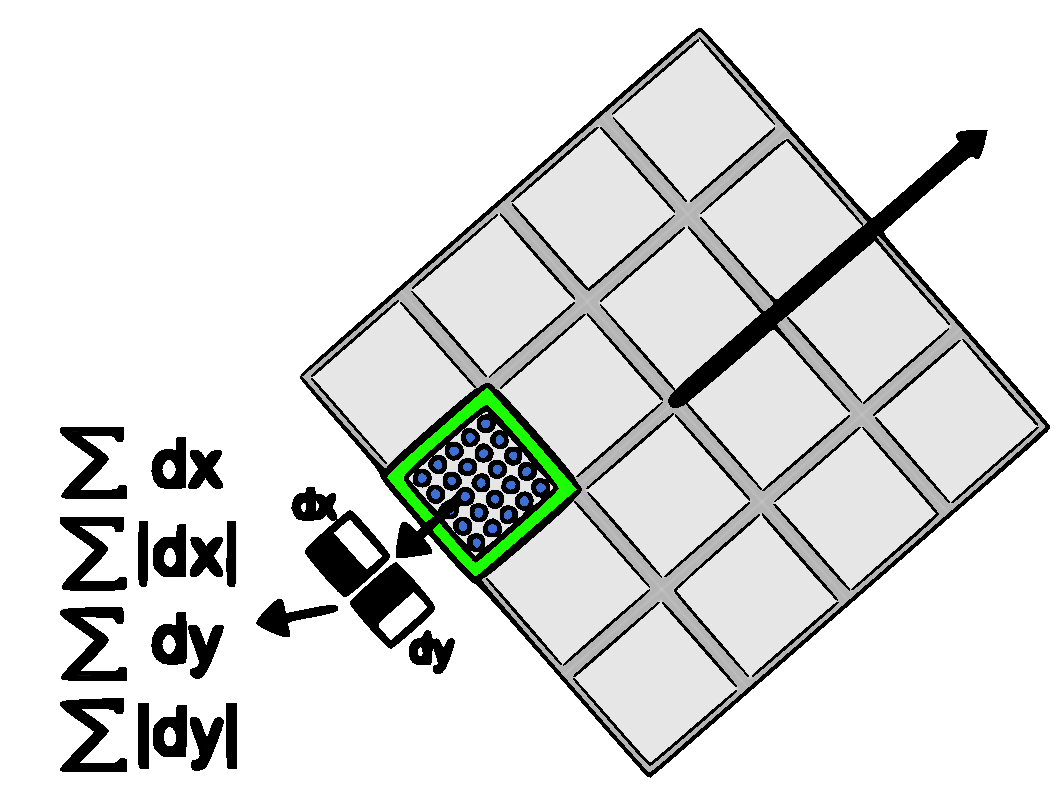
\includegraphics[width=\columnwidth]{2.mainmatter/2.Methodology/FeaturesExtraction/figures/SURF/descriptor-components}%
	   \caption[Descriptor Components]{Descriptor Components.  \imgsrc{(Image source: Evans~\cite{Evans:09})}}%
	   \label{fig:descriptor-components}%
\end{figure}	
	
	
\end{itemize}


\end{enumerate}
\newpage 
\section{Experimental Results}
\label{sec:results-feature-extraction}
In this section, I will present experimental results on feature extraction and reason for choosing specific algorithm. I used Intel \emph{OpenCV (Open Source Computer Vision)} library version 2.3 to test the performance of the feature extractors. I developed the algorithms using \emph{C++} in \emph{Microsoft Visual Studio 2010}. I carried out tests in my machine with following configurations:
\begin{itemize}
	\item Operating System: Windows 7 Professional 64 bit
	\item Processor: Intel Core i5 2.80 GHz
	\item Memory: 8.00 GB 	
\end{itemize}

I will focus on the following two measures to select best algorithm:
\begin{description}
\item[Accuracy] The inaccurate stitching result may give false information to the analysts; we choose the algorithm which results best accuracy for medical images. I will check the stability of the detected corners for different intensity, orientation, and scaling.
\item[Computational Complexity] High computational complexity will take longer time to perform a task which is undesirable. We try to get the algorithm which has real time performance. Sometimes, we tweak the algorithms to work faster (parallel processing for example). There is trade-off between computational complexity and accuracy. So, we select the algorithm which is faster and gives acceptable result. 
\end{description}

\noindent I have tested 3 popular feature extractors: Harris, SIFT and SURF. A good corner detector should fulfill certain requirements as discussed in section~\ref{sec:req-corner-detector}, so I will evaluate the feature detectors based upon those requirements i.e. computational time and repeatability rate of key-points for different intensity, orientation, scaled images.\\

\noindent To evaluate the performance of the detectors, I have used the different images mentioned below:
\begin{description}
\item[Normal Image] This is normal X-ray image of resolution 666 x 1024 (i.e. 681984 pixels). This is standard image and I have modified this image to create other different intensity or orientational images. 

\item[High Intensity Image] The pixels of the normal image are increased by 25\% to get high intensity image. The high intensity image and normal image have same number of pixels.
\item[Rotated Image] The normal image rotated by 8\deg and the unassigned pixels have been removed and the image size is 538 x 892 (i.e. 479896 pixels). Thus, the rotated image pixels have been reduced by 30\%.
\item[Scaled Image] The height and width of the normal image are increased to get scaled image. The resulting scaled image size is 1138x1751 (1992638 pixels) which contains nearly double the pixels in the normal image.
\item[Noisy Image] The normal image consists of very little noise. To carry out the tests for noise image, I have added some Gaussian noise (with mean=0, variance=0.001) to the standard image to get the noisy image.
\end{description}

\subsection{Experiment 1: Computational Time}
% Data: Harris: 72.714 54.013 38.076 158.564 53.619
       %SIFT: 402.993 350.434 270.318 1019.413 379.934
			 % SURF: 242.045 240.767 177.066 705.498 244.308                                             
I have estimated the computational time for the feature extractors for different intensity and orientation images mentioned above. The computational time of the key-point detectors has been presented in chart
%measurement(in milliseconds) is presented in table~\ref{table:feature-computational-time} and the chart is 
shown in figure~\ref{fig:feature-computational-time}. \\
%\begin{table}[H]
%\begin{tabular}{l|c|c|c|c|c|}
%\cline{2-6} 
%& \multicolumn{5}{c}{Computing Time(milliseconds)}\\ \cline{2-6}
%& Original & High Intensity  & Rotation & Scale & Noise \\ \hline
%\multicolumn{1}{|c|}{Harris} & 72.714 & 54.013 & 38.076 & 158.564 & 65.919\\ \hline
%\multicolumn{1}{|c|}{SIFT} & 402.993 & 350.434 & 270.318 & 1019.413 & 427.934\\ \hline
%\multicolumn{1}{|c|}{SURF} & 242.045 & 240.767 & 177.066 & 705.498 & 240.308\\ \hline 
%\end{tabular}
%\caption{Computational time of feature detectors}
%\label{table:feature-computational-time}
%\end{table}

\begin{figure}[H]%
\centering
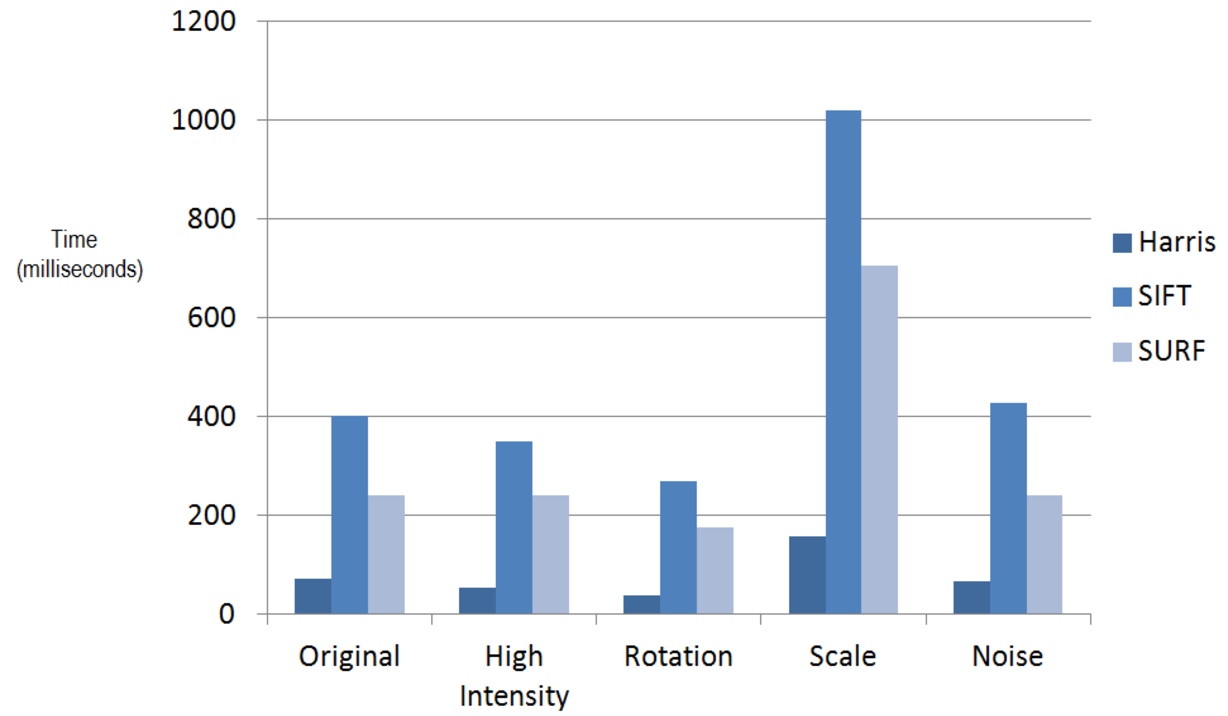
\includegraphics[width=\columnwidth]{2.mainmatter/2.Methodology/FeaturesExtraction/figures/features-CT}%
\caption[Comparison: Computational Time]{Chart showing the computational time (milliseconds) of feature extractors for different images}%
\label{fig:feature-computational-time}%
\end{figure}

\noindent The original, high intensity and noisy images contain same number of pixels; the time taken by the detectors seems similar for those images. For rotated image, the pixels are reduced by 30\%, the computational time also decreases. Similarly, the detectors are slower for scaled image because it contains almost double the number of pixels in original image.\\

\noindent The chart shown in figure~\ref{fig:feature-computational-time} clearly reveals that Harris corner detector is the fastest among detectors and SIFT is the slowest for all types of images. Keeping this in  mind, we go on further experiments to evaluate the accuracy of the feature detectors to figure out the best feature extractor.


\subsection{Experiment 2: Stability}
In this experiment, the stability of the feature detectors is computed for different intensity or orientation images. The stability of the key-point detectors is an important property because it determines the accuracy of the detected key-points. To measure the stability of a key-point detector, we apply key-point detecting algorithm to the standard image (i.e. normal image) and other images; then count the number of key-points. The repeated key-points lie on the same feature location of the standard image. The repeated key-points on the other images are counted. Suppose, we got $N$ key-points in standard image and $N'$ key-points in other image; out of which $N_{repeated}$ are repeated. We estimate the stability of the key-point detector as follows:
\begin{equation}
Stability=\frac{N_{repeated}}{N}
\label{eq:stability}
\end{equation}
The stability is generally expressed in percentage (\%) and the higher the stability the better is the key-point detector. So, we select the feature detector which gives highly stable corners.\\ 

\noindent Table~\ref{table:corners-count} presents the detected key-points count for original image and other variant images. I have included the counts for repeated key-points to estimate the stability of the feature detector.
\begin{table}[H]%
\centering
\begin{tabular}{l|c|c|c|c|c|c|}
\cline{2-7}
&\multicolumn{2}{|c|}{\textbf{HARRIS}} & \multicolumn{2}{|c|}{\textbf{SIFT}} & \multicolumn{2}{|c|}{\textbf{SURF}} \\ \cline{2-7}
& \multicolumn{2}{|c|}{Original image: 245} & \multicolumn{2}{|c|}{Original image: 306} & \multicolumn{2}{|c|}{Original image: 291} \\ \hline
\multicolumn{1}{|c|}{\textbf{Image}} & \textbf{Identified} & \textbf{Repeated} & \textbf{Identified} & \textbf{Repeated} & \textbf{Identified} & \textbf{Repeated} \\ \hline
\multicolumn{1}{|c|}{Brighter} & 183 & 136 & 261 & 225&255 & 234\\ \hline
\multicolumn{1}{|c|}{Rotated} & 173 & 85 & 196 & 139& 177 &125\\ \hline
\multicolumn{1}{|c|}{Scaled} & 481 & 82 &265 & 259& 299 & 164 \\ \hline
\multicolumn{1}{|c|}{Noisy} & 273 & 174 & 488 & 290 & 325 & 214 \\ \hline
\end{tabular}
\caption[Feature Points Count]{Feature points count for stability measurement}
\label{table:corners-count}
\end{table} 

\noindent The count of generated and repeated key-points of the images are used to compute the stability of the feature extractors (using equation~\ref{eq:stability} above). The stability of the key-point detectors for different images has been  presented in chart shown in figure~\ref{fig:repeatability-chart}.

%\begin{table}[H]%
%\centering
%\begin{tabular}{ll|c|c|c|}
%\cline{3-5}
 %&& HARRIS & SIFT & SURF\\ \cline{1-5}
%\multicolumn{1}{|c|} {\multirow{4}{*}{\textbf{Stability(\%)}}} & Brighter & 55.51 & 73.52& 80.41\\ \cline{2-5}
 %  \multicolumn{1}{|c|}{}& Rotated & 34.69 & 45.42& 42.96\\  \cline{2-5}
%		\multicolumn{1}{|c|}{}& Scaled & 33.46 & 84.64 & 56.35 \\ \cline{2-5}
%		\multicolumn{1}{|c|}{}& Noisy & 71.02 & 94.77 & 73.53\\ \hline	
%\end{tabular}
%\caption[Stability measurement]{Stability measurement of the corner detectors}
%\label{table:stability}
%\end{table}


\begin{figure}[H]%
\centering
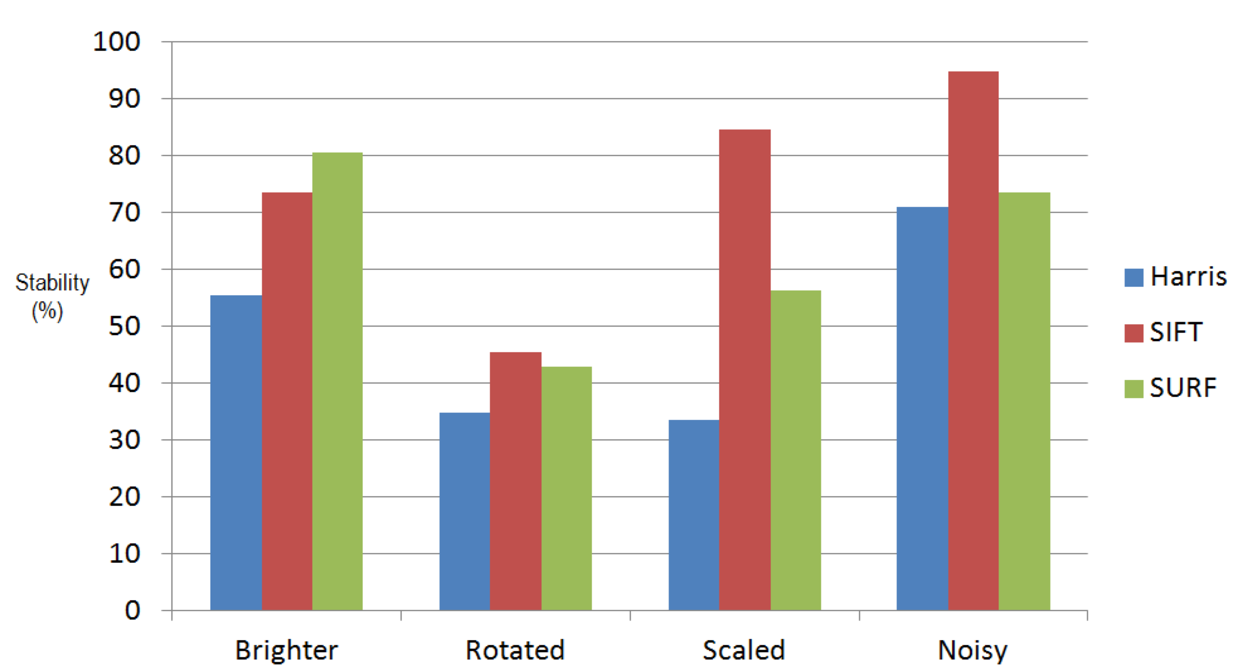
\includegraphics[width=\columnwidth]{2.mainmatter/2.Methodology/FeaturesExtraction/figures/feature-extraction-stability}%
\caption[Comparison: Stability of Corners]{Chart showing the stability of  feature extractors}%
\label{fig:repeatability-chart}%
\end{figure}

\noindent The chart presented in figure~\ref{fig:repeatability-chart} shows that SIFT has high stability for all types of images while Harris giving low stable corners. It is interesting that all key-point detectors have high stability for noisy image. It is because the detectors generate very large number of key-points for noisy image (see table~\ref{table:corners-count}). Therefore, we get higher number of repeated key-points which results higher stability. The less stable key-points for rotated images is because of the decreased size of rotated image i.e. some part of the rotated image is trimmed off to remove unassigned pixels.\\

\noindent In conclusion, Harris corner detector is computationally efficient; but produces less stable key-points which means it generates more inaccurate or inconsistent key-points for different intensity or orientational images. Stability is an important feature for key-point detectors and SIFT and SURF are good to generate highly stable key-points. SIFT is slower but giving highly stable key-points while SURF is faster but less stable than SIFT. So, both SIFT and SURF are chosen as the good key-point detectors. In the next chapter, we will evaluate the matching performance of SIFT and SURF.

%Include the picture of SIFT and SURF with different rotations and scaling. Show the repeatibility with matching points.

% Include the time measure of SIFT and SURF

% Present the comparison chart of Harris, SIFT and SURF




\chapter{Features Matching}
\label{chapter:feature-matching}
The next step after feature extraction is feature matching. As explained in section~\ref{sec:feature-extraction}, we will get a set of key points and their descriptors for each image. The matching process uses the descriptor information to find out the corresponding matching points in the images. All the points in one image are compared to all the points in other image and best matched point is identified. The nearest-neighborhood based algorithms are basically used for feature matching and since those methods are slower, we have to optimize to get the faster matching. The first section of this chapter gives exhaustive \emph{k-nearest-neighborhood (kNN)} method, then we discuss \emph{approximate nearest neighborhood (ANN)} method in the following section. The fine-tuning of the matching points has been described in last two sections.    

\section{kNN Matching}
\label{sec:knn-matching}
 The k-nearest neighbor (kNN) search problem is widely used in classification problem. If we have a set $P$ of reference points $P=\left\{ p_1,p_2, p_3,...,p_m \right\}$ in $d$-dimensional space, and suppose $q$ be the query point defined in the same space, then kNN search problem determines the $k$ points closest to $q$ among $P$ as shown in figure~\ref{fig:knn-search}.  

\begin{figure}%
\centering
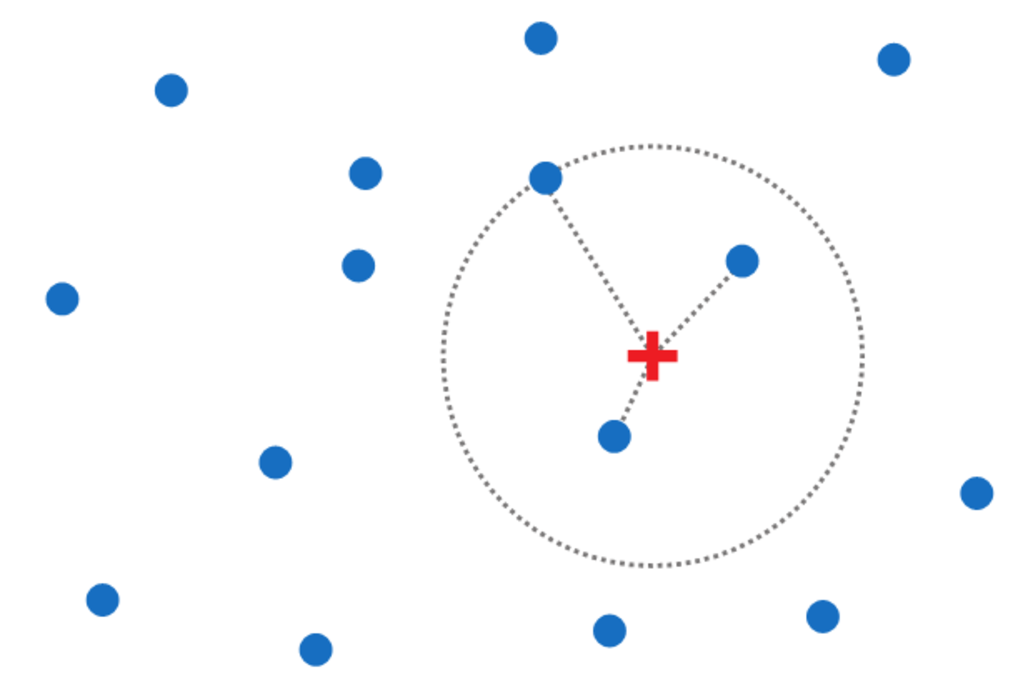
\includegraphics[width=0.6\columnwidth]{2.mainmatter/2.Methodology/figures/Knn}%
\caption[kNN Search]{kNN search problem with k=3. \imgsrc{(Image source: Garcia et al.~\cite{Garcia:10})}}%
\label{fig:knn-search}%
\end{figure}

\section{ANN Matching}
\label{section:ann-matching}
Since, we have high dimensional feature vector \footnote{Each SIFT point has 128 features while a SURF point has 64 features}, and obviously we will have a lot of key points. So, in image stitching problems, exhaustive matching process (such as kNN) is very slow, we select an alternative approximate nearest neighborhood matching i.e. \emph{ANN Matching} where priority-search is carried out on hierarchical k-means trees~\cite{muja:09}. The nearest points need not necessarily be the actual matched points, further tests are necessary to increase matching accuracy (e.g. Ratio Test, Symmetry Test).\\

\noindent The ANN algorithms can be orders of magnitude faster than kNN search, and provides nearest optimal accuracy~\cite{muja:09}. 


\section{Removing False Matches}
The nearest neighborhood based feature matching techniques mentioned above might contain a lot of false matches. Before we go for estimation of transformation parameters, we have to remove those false matches. This section describes the two effective methods to remove false matches: \emph{Ratio Test} and \emph{Symmetry} Test~\cite{Laganière:11}. 
\subsection{Ratio Test}
\label{sec:ratio-test}
For kNN search, if we set $k=2$, the matching finds the two nearest points. The ratio test is based upon the ratio of distances of the two nearest points. Suppose $d_1$ and $d_2$ ($d_1<d_2$) be the distances of a point to its nearest matched points, and a we define a threshold $T$. Then, we reject the points as false matches which satisfy the following condition:
\begin{equation}
\frac{d_1}{d_2}>T
\label{eq:ratio-test}
\end{equation}
If two nearest points are almost same distance, the ratio tend to be higher which implies the false matches, so ratio test confirms the nearest point should be very near and other point should be far. To what extent we remove the points depends upon the threshold $T$ selected i.e. higher the threshold, larger number of matches. Generally, we select $T$=0.8 i.e. if the distance ratio between the two nearest points is greater than 0.8, then ratio test discards that matching pair. Generally, we get more accurate matches by decreasing threshold value; but this is not always true. In some cases, if the image contains similar points (i.e. $d_1 \approx d_2$) in different locations, then ratio $\frac{d_1}{d_2}$ for a match might be higher than threshold ($T$) and the match is discarded.


\subsection{Symmetry Test}
\label{sec:symmetry-test}
In symmetry test, we compute the matches between the images in both direction and select the matches which pass the symmetry test i.e. any matching pair should be symmetrically valid to be accurate match; otherwise the match is discarded as false match. This is very effective test to identify the false matches and we generally prefer to carry out this test after ratio test.\\

\noindent Suppose, a key-point $p_1$ in the first image gets a matched point $p_1'$ in the second image, then match pair \{$p_1$, $p_1'$\} to be an accurate match, the key-point $p_1'$ in the second image should have matched point $p_1$ in the first image. If $p_1'$ gets other key-point as matched point then \emph{Symmetry Test} discards the matched pair \{$p_1$, $p_1'$\}. This test is simple to implement and we do not need any parameters to perform this test.

\newpage
\section{Experimental Results}
\label{sec:feature-matching-experimental-result}
In this section, I will evaluate the feature matching methods in term of computational complexity. Section~\ref{sec:SIFT-SURF} compares SIFT and SURF features matching and section~\ref{sec:kNN-ANN} compares the nearest neighborhood methods (i.e. kNN and ANN) for feature matching. 

\subsection{SIFT versus SURF}
\label{sec:SIFT-SURF}
To carry out the evaluation between SIFT and SURF, I varied the number of feature points in first image by changing threshold values while the number of feature points in the second image made fixed with constant threshold value. The chart presented in figure~\ref{fig:chart:SIFT-SURF} shows that SURF is quite faster than SIFT. The computational cost for SIFT increases drastically as the number of points increases. I used exhaustive kNN matching to match the features.
\begin{figure}[H]%
\centering
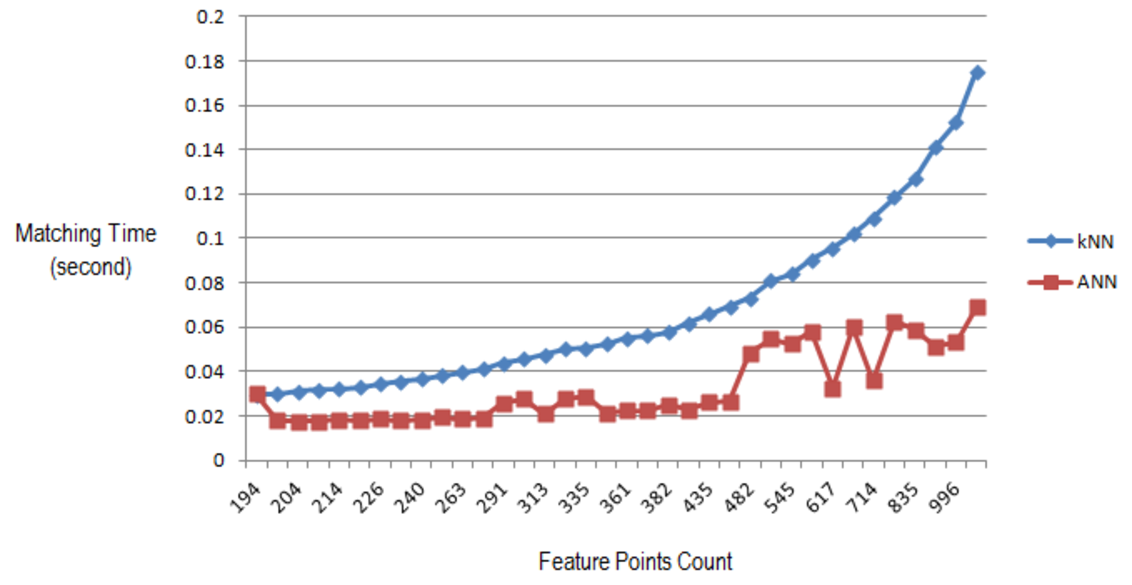
\includegraphics[width=1.2\columnwidth]{2.mainmatter/2.Methodology/figures/SIFT-SURF}%
\caption[Comparison of SIFT and SURF]{Comparison of SIFT and SURF: Feature points versus computational time}%
\label{fig:chart:SIFT-SURF}%
\end{figure}

\noindent SIFT is more accurate because of its high dimensional features, its high computational time is the main drawback making it inappropriate for real time or user-centered applications like medical software. I have chosen SURF method because it is faster and still it gives accurate matches. 

\subsection{kNN versus ANN}
\label{sec:kNN-ANN}
In this section, I will present experimental results on kNN and ANN matching methods for SURF features (64 dimensions) which is presented in graph shown in figure~\ref{fig:knn-ann}. The graph clearly shows that ANN matching always faster than kNN. kNN matching is showing exponential increase in computational complexity when key-points are increased which implies that kNN becomes expensive for large key-points. In practice, we have larger number of feature points to be matched, so ANN matching is preferred to kNN.

\begin{figure}[H]%
\centering
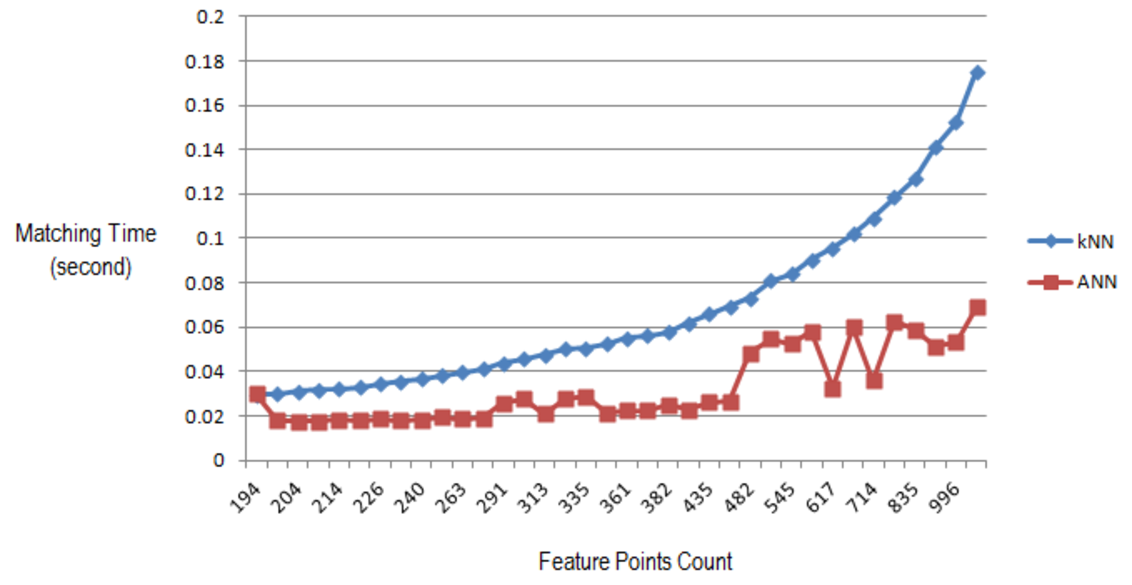
\includegraphics[width=1.3\columnwidth]{2.mainmatter/2.Methodology/figures/kNN-ANN}%
\caption[Comparison of kNN and ANN]{Comparison of kNN and ANN: Feature points vs. matching time}%
\label{fig:knn-ann}% 
\end{figure}

\subsection{Getting Accurate Matches}
\label{sec:accurate-matches}
The nearest neighborhood method just gives the closest point as the matching point which is not necessarily the true match. So, we have to implement tests to remove the false matches identified by nearest neighborhood method. In this section, I implemented some tests to increase the accurate matches by identifying possible false matches. The increment of accurate matches helps to get more accurate transformation model (i.e. \emph{homography}).\\ 

\noindent I have implemented \emph{Ratio} (section~\ref{sec:ratio-test}) and \emph{Symmetry} (section~\ref{sec:symmetry-test}) tests and presented the results in graphical form as shown in figure~\ref{fig:accurate-matches}. The ANN matching resulted 1295 matches (figure~\ref{fig:matches-nn}) , then a significant number of inaccurate matches (1118 matches) are removed by Ratio test (figure~\ref{fig:ratio-test}). For remaining 177 matches, I carried out Symmetry test, which again removed 80 inaccurate matches to get 97 best matches as shown in figure~\ref{fig:symmetry-test}. Although these tests removed significant number of inaccurate matches, the obtained best matches are not 100\% accurate which we can be clearly seen in figure~\ref{fig:symmetry-test}. The remaining inaccurate matches can be identified as outliers by robust estimation methods discussed in the next chapter.


\begin{figure}[H]%
\begin{center}
\subfloat[Nearest neighborhood matches]{\label{fig:matches-nn} 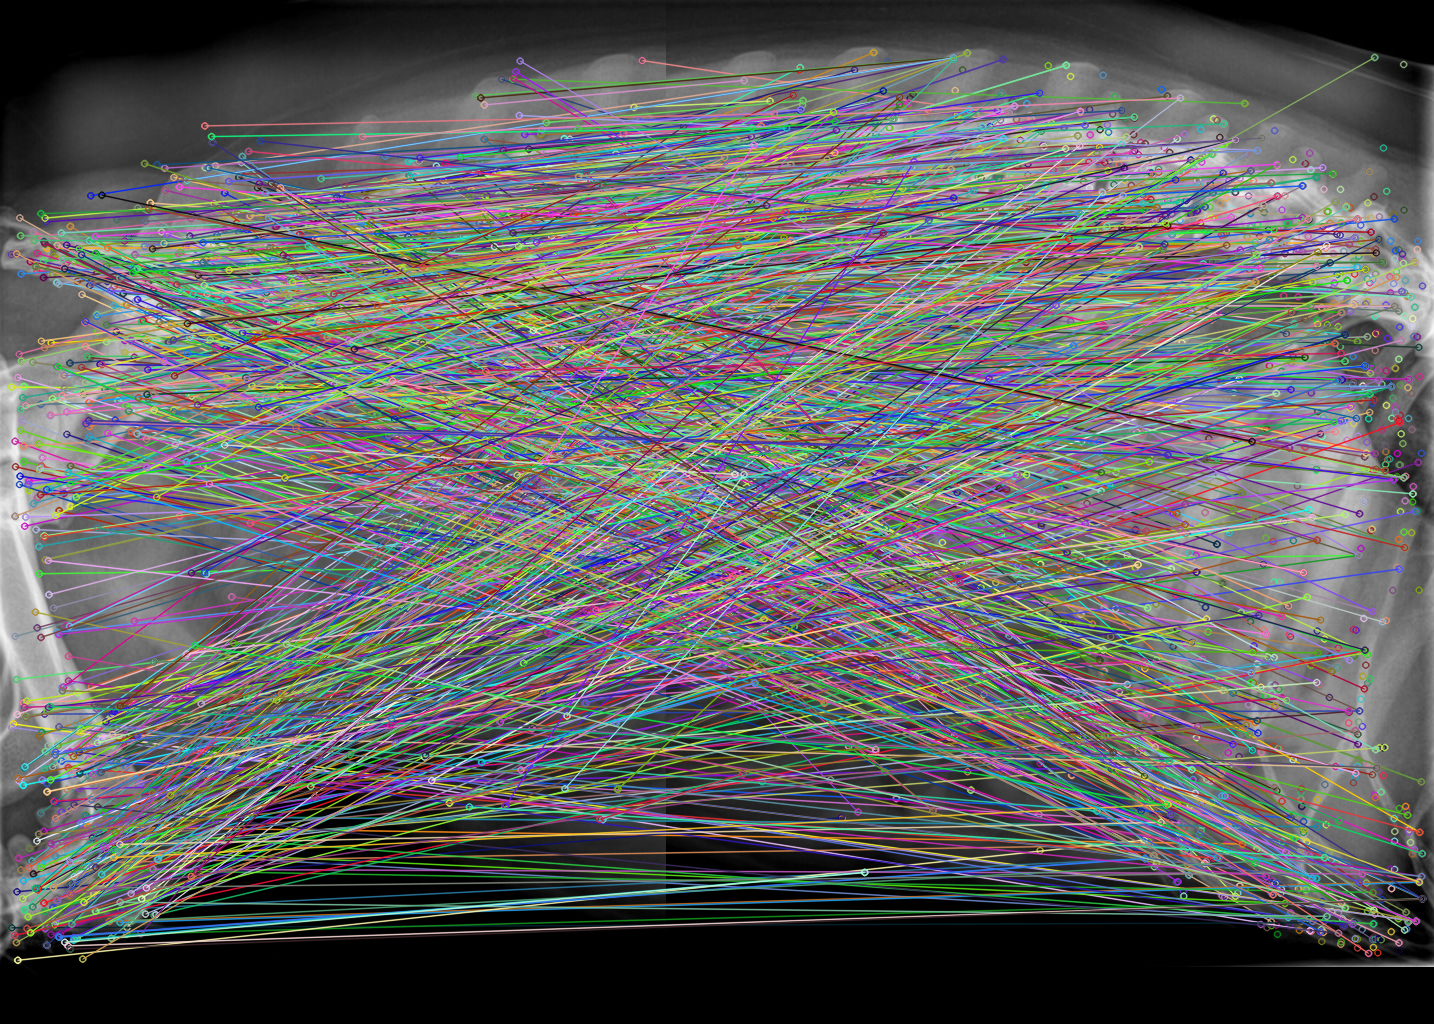
\includegraphics[width= 0.70\columnwidth]{2.mainmatter/2.Methodology/figures/matches}} \hspace{1mm}
\subfloat[Ratio Test] {\label{fig:ratio-test} 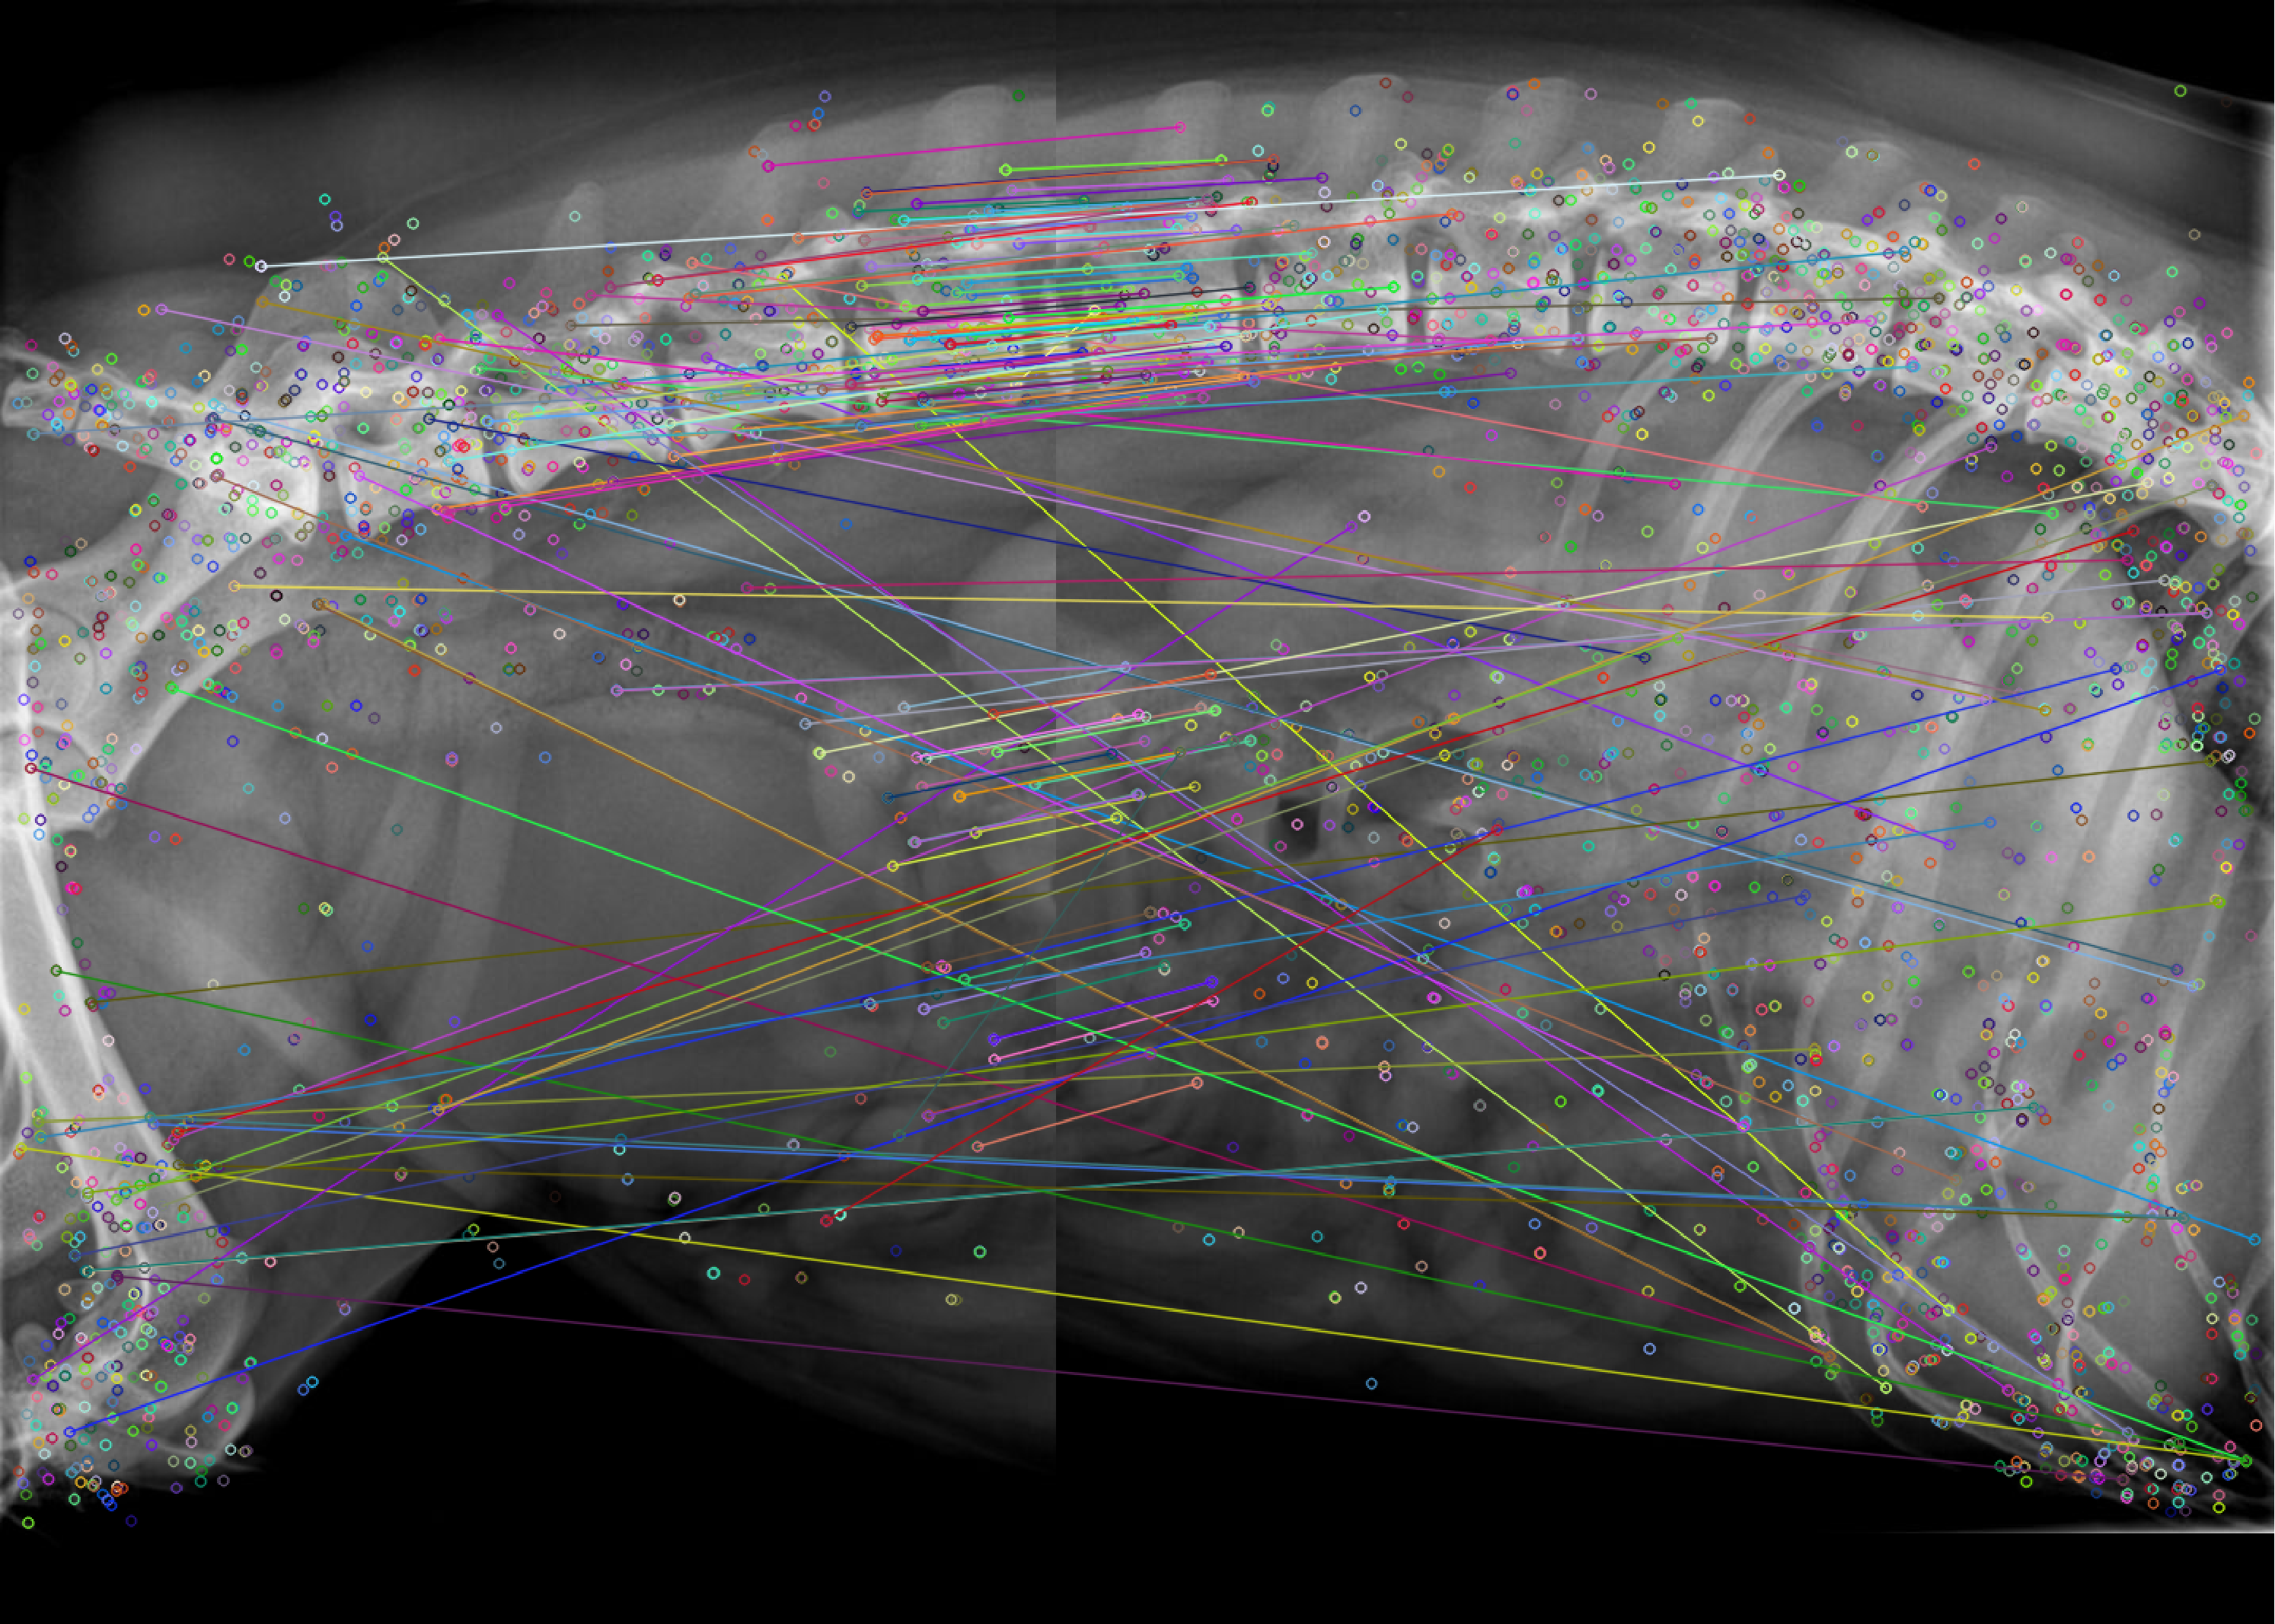
\includegraphics[width= 0.70\columnwidth]{2.mainmatter/2.Methodology/figures/ratio-test}}\quad
\subfloat[Symmetry Test] {\label{fig:symmetry-test} 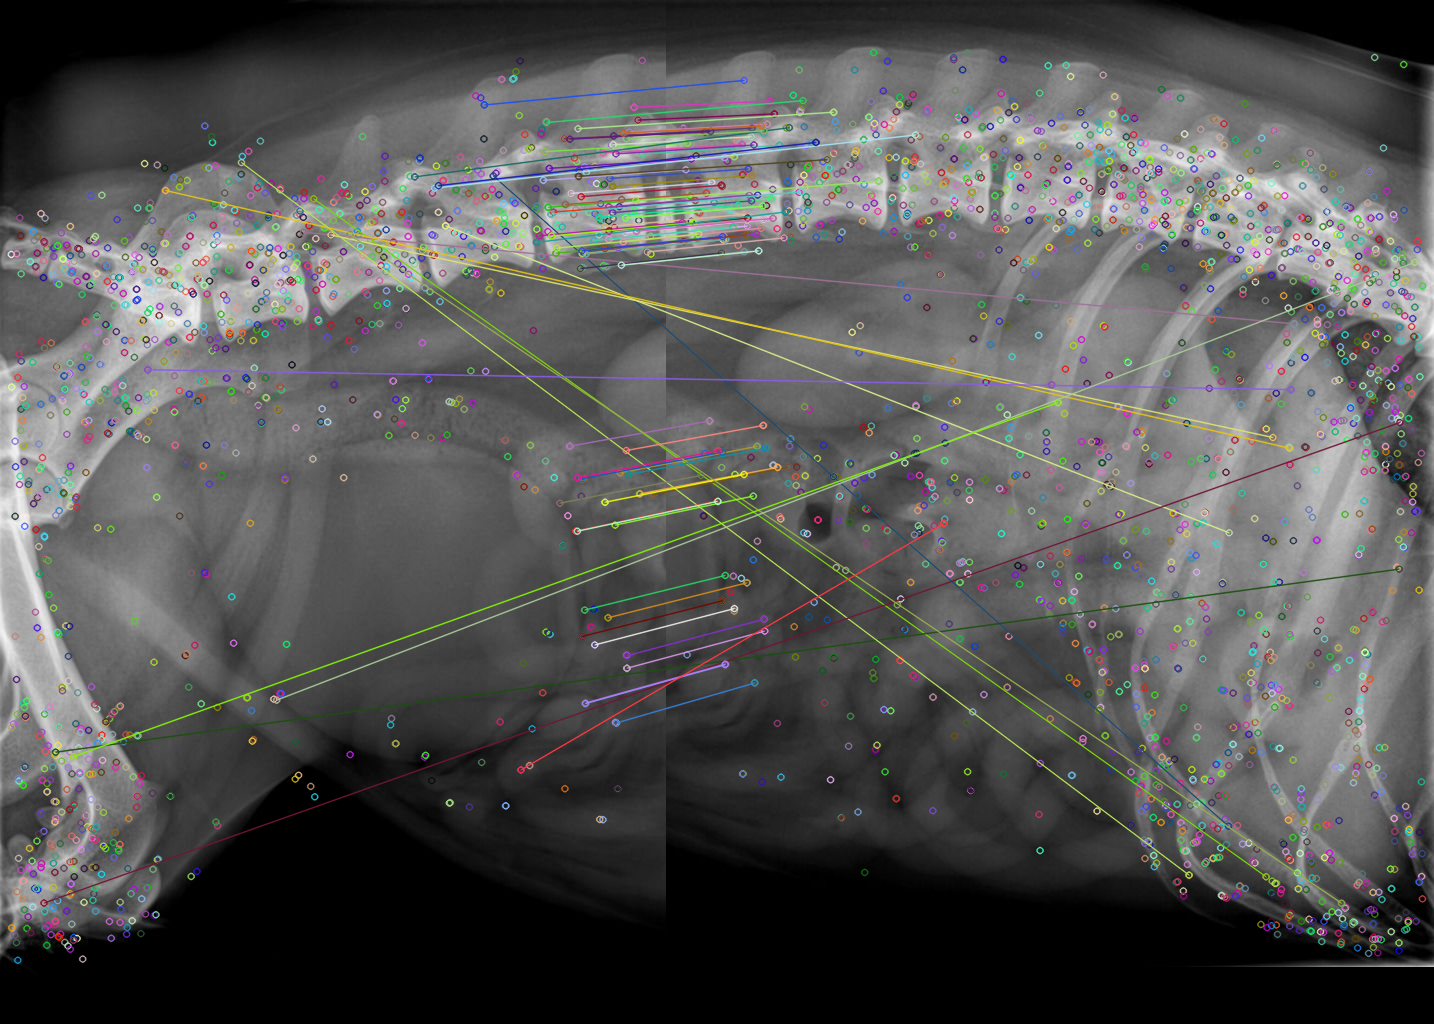
\includegraphics[width= 0.70\columnwidth]{2.mainmatter/2.Methodology/figures/symmetry-test}}
\caption[Steps of Getting Best Matches]{Steps of getting best matches:~\subref{fig:matches-nn} a lot of matches found using NN method~\subref{fig:ratio-test} Ratio test removed a significant number of false matches.~\subref{fig:symmetry-test} The false matches from ratio test are further removed by symmetry test.}%
\label{fig:accurate-matches}%
\end{center}
\end{figure}






\chapter{Homography Estimation}
\label{chapter:homography-estimation}
This chapter discusses about the estimation of transformation model using matches estimated in previous chapter. The best matches we estimated still not guaranteed to be true matches, so there may be chances of getting wrong motion parameters if we include such false matches to estimate motion model. We use homography matrix as motion model for transformation. We use robust methods to estimate homography which uses only true matches.\\

\noindent If there is only translation or rotation between the images to be stitched, then stitching process will be simpler; we need only affine transformation parameters. The real problems will be to register images obtained using different camera angle; we have to estimate translation, rotation and projection parameters which can be represented by estimating \emph{homography matrix}.\\

\noindent A homography is a 3x3 matrix $H$ and the elements of the matrix contains the rotation, translation and projection parameters. We can change the value of homography $H$ without changing the projective transformation. Therefore, $H$ can be considered as homography matrix and it has 8 degrees of freedom (although it has 9 elements)~\cite{Dubrofsky:07}. In other words, we need to solve for 8 unknowns to get the homography matrix. 


\section{Algorithm for homography Estimation}
The homography matrix is solved using \emph{Direct Linear Transform (DLT)} algorithm if we have sufficient set of point correspondences. We solve the homography matrix by using the following equation:
\begin{equation}
x_i'=Hx_i
\label{eq:homography-estimation}
\end{equation}
where $x_i$ and $x_i'$ are 3 element vectors. For stitching problem, we use the corresponding points as vectors. In 2D problem, suppose, $\textbf{x}= (x,y,1)^T$ and $\textbf{x'}= (x',y',1)^T$ are two corresponding points, then the relationship will be
\begin{equation}
c\left(
\begin{array}{c}
	x \\
  y \\
	1	
\end{array}
\right)
=H \left( 
\begin{array}{c}
	x' \\
	y' \\
	1
\end{array}
\right)
\label{eq:homography-estimation-detail}
\end{equation}
Hartley and Zisserman~\cite{hartley:04} suggested to use a normalization step in DLT because the DLT algorithm is dependent on the origin and scale of co-ordinate system of the image. The normalized DLT algorithm can be summarized by the following steps:
\begin{enumerate}
	\item Translate the points such that the centroid lies at the origin. 
	\item The scaling of the points is carried out to maintain their average distance to be $\sqrt{2}$.
	\item Get transformations for both the images independently and apply DLT algorithm to get homography matrix. 
\end{enumerate}
For more detail algorithm, it is suggested to study chapter 4 of Hartley and Zisserman book~\cite{hartley:04}


\section{Robust Estimation}
\label{section:robust-estimation}
The homography estimation requires 4 corresponding points, and the matching methods described in previous sections are not robust i.e. there may be chances of some false correspondences. The two features in the images might not correspond to same the real feature. So, we need to identify the inlier and outlier correspondences and only inlier matches can be used for homography estimation. This section discusses two most popular methods for homography estimation.
%RANSAC%
\subsection{RANSAC}
\label{sec:ransac}
RANSAC (Random Sample Consensus) was first purposed by Fischler~\emph{et~al}~\cite{fischler:81} and it is the most commonly used robust estimation method for homographies~\cite{Dubrofsky:07}. This method selects 4 correspondences randomly and computes homography matrix $H$. Then other correspondences are classified as inliers or outliers depending on its concurrence with $H$. This process is repeated for a number of iterations and the iteration which gives largest number of inliers is identified. The homography $H$ for that iteration is chosen as the best transformation model.\\

\noindent The classification of inliers or outliers is carried out by assigning some distance threshold $t$ and if $\|\textbf{x'} - H\textbf{x}\| > t$, then the point is considered as outlier. The threshold value is problem specific. The higher the threshold value, the larger the inliers we get. Similarly, we choose a number of iterations $N$ so that at least one of the random samples will be free from outliers\footnote{We have to test each combination of random samples, so we need to limit the number of iterations}. Hartley and Zisserman~\cite{hartley:04} derived a formula to compute the number of iterations required for RANSAC:
\begin{equation}
N=log(1-p)/log(1-(1- \epsilon)^s)
\label{eq:number-of-iterations}
\end{equation} 
where $p$ = probability at least one of the samples is free from outlier. We generally use p=0.99\\
$\epsilon$=probability of outlier which can be expressed as 
\begin{equation}
\epsilon= 1- \frac{number\_of\_inliers}{total\_number\_of\_points}
\label{eq:outlier-probability}
\end{equation}
$s$ =number of correspondences used in each iteration. ($s=4$)\\

\noindent Hartley and Zisserman~\cite{hartley:04} \footnote{see comparison table in chapter 4 of the literature.} claims that if we have 5\% outliers(i.e. $\epsilon$=0.05) then only 3 iterations are needed to get at least one pure sample with probability=0.99.

%LMS%
\subsection{Least Median of Squares Regression}
\label{sec:least-median-square}
In RANSAC, we use distance threshold to identify outliers and exclude them for homography estimation. This method, as the name suggests, calculates the median of squares of the error value (i.e. difference between transformed and actual points) for each point in each iteration. The best homography is the one which gives least median value.\\

\noindent The Least median of Squares (LMS) was first introduced by Peter J. Rousseeuw~\cite{rousseeuw:84} and he claims that the estimator can resist the effect of nearly 50\% of contamination in the data. The ordinary least squares (OLS) estimators can not identify the non normal errors, so, LMS estimator is claimed to be a robust~\cite{rousseeuw:84}~\cite{onder:01} and it has the characteristics of being highly resistance to high proportion of outliers~\cite{onder:01}.\\

\noindent So, in summary, LMS is an effective method to detect the outliers. We do not need any initial parameters (unlike $t$ and $\epsilon$ in RANSAC). The only disadvantage of this method is that it can not work well if there are more than half outliers.  

\newpage
\section{Experimental Results}
% Select Ransac, because we are not sure that more than half of the keypoints are inliers
The first part of this section presents the result of RANSAC for homography estimation by identifying outliers. While LMS method (section~\ref{sec:least-median-square}) works good when there are more than 50\% inliers, it is not always guaranteed to have more than half accurate matches\footnote{there might be chances of being more false matches since we have used less accurate methods like SURF and ANN to get faster result}, so I prefer RANSAC method for robust estimation and it works even if there are large number of outliers. The equation~\ref{eq:number-of-iterations} reveals that we need few iterations to get a pure sample with high probability even if there are a lot of outliers.\\

\noindent In the next section, I include experiment on the effect of distance threshold value ($\sigma$) to the number of inliers or outliers.  The distance threshold $\sigma$ has been measured in pixels. 

\subsection{Robust Estimation with RANSAC}
For RANSAC, I have set the maximum possible number of iterations ($N$) up to 2000 and distance threshold ($\sigma$) 2 pixels. After some iterations, I got inliers (accurate matches), outliers (inaccurate matches) and the homography matrix $H$. Figure~\ref{fig:RANSAC-result} shows the inlier matches after I obtained using RANSAC method. From the figure, we can easily see that the all inliers are true matches.

\begin{figure}[H]%
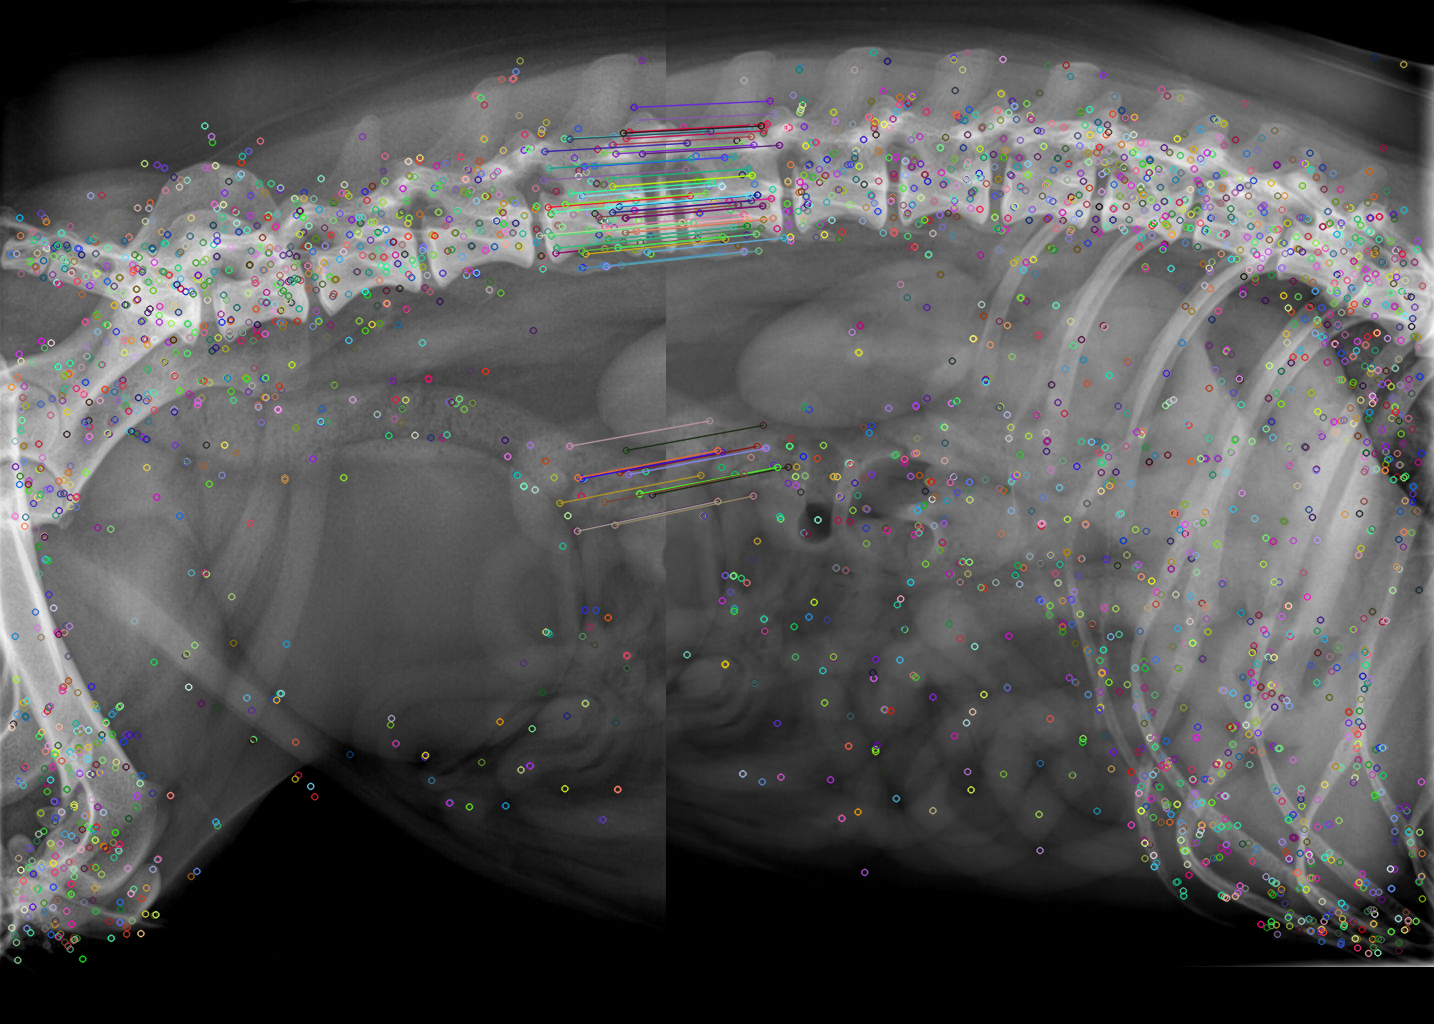
\includegraphics[scale=0.25]{2.mainmatter/2.Methodology/figures/inliers}
\caption[Matches After Removing Outliers]{Matches after removing outliers ($\sigma$=3 pixels). This figure shows all matches are accurate.}%
\label{fig:RANSAC-result}%
\end{figure}

\subsection{Effect of Distance Threshold ($\sigma$)}
The number of inliers is changed when we change the distance threshold $\sigma$. This section includes experiment on the effect of $\sigma$ to the number of inliers we obtained. The graph presented in figure~\ref{fig:inliers-vs-distance-threshold} shows that increase of $\sigma$, increases the number of inliers. So, we have to select proper $\sigma$ so that all inliers are true matches. With small possible value of $\sigma$=1 pixel, I got 50 inliers. Since the figure~\ref{fig:RANSAC-result} shows there are 62 accurate matches which implies that $\sigma$ = 1 is missing some true matches. The increase of $\sigma$ increases the inliers which also increases probability of including false matches as inliers. So, the best accepted values of $\sigma$ seems to be either 1 or 2. 

\begin{figure}[H]%
\centering
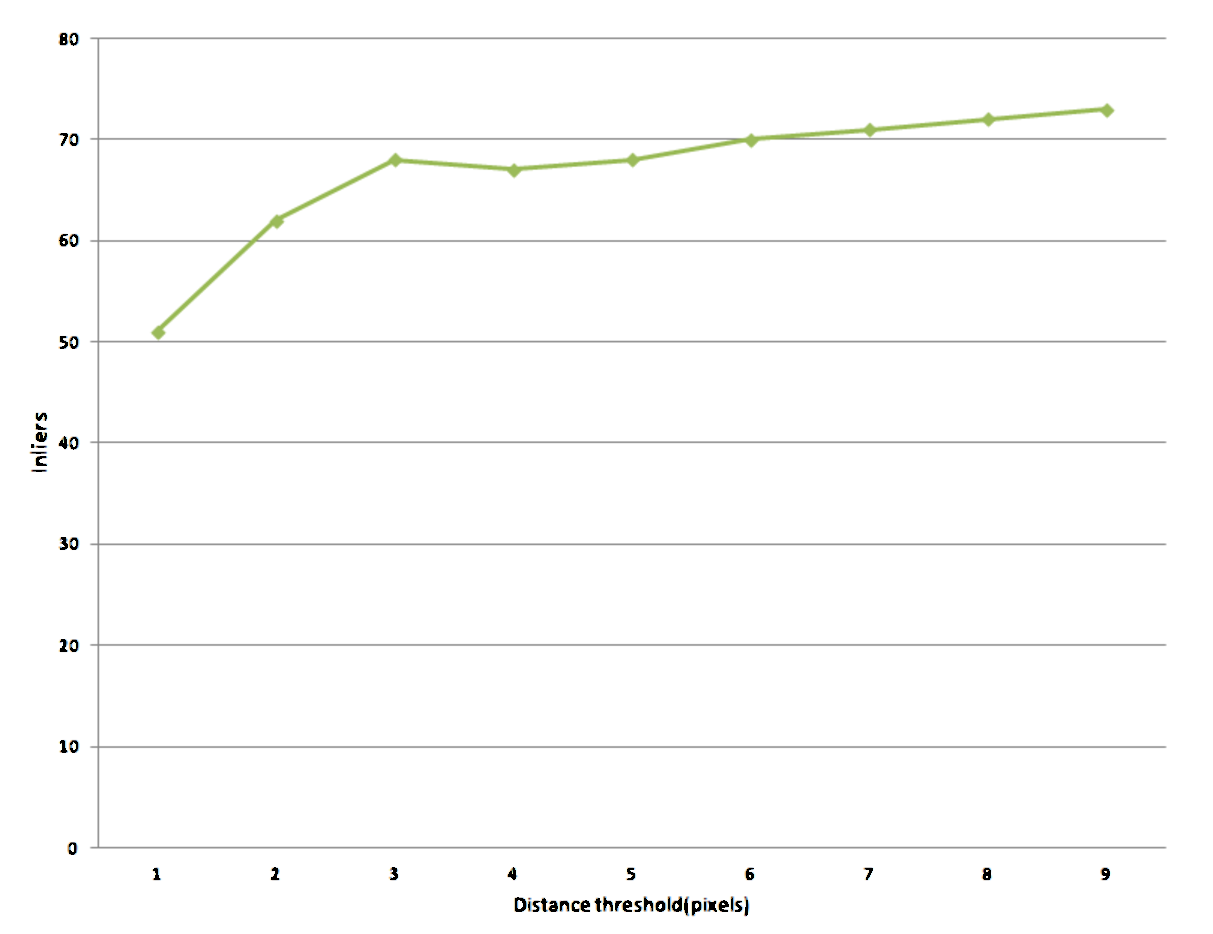
\includegraphics[width=1.0\columnwidth]{2.mainmatter/2.Methodology/figures/Inliers-threshold}%
\caption[Distance Threshold and Inliers Count]{Graph showing inliers versus distance threshold}%
\label{fig:inliers-vs-distance-threshold}%
\end{figure}

\noindent In some cases, if the stitching X-ray images are not exactly same, then key-points do not go with the transformation model (i.e. $H$) which results very few or sometimes insufficient inliers to guarantee the accuracy of homography. In that situation, we increase $\sigma$ value to get more inliers while estimating homography.\\

\noindent The number of inliers \footnote{The inliers in this context is the best inliers we got after a number of iterations.} can also be used to identify the feasibility of stitching between two images. There might be cases when we try stitching images which do not have any common region. The inliers are counted to confirm whether the images can be stitched. We define any number greater than sample size. Most of the time, if we have more than 15 inliers, we accept the homography to create composite image. For very few inliers\footnote{Few inliers imply limited or no overlapping between input images.}, there is chances of getting inaccurate homography and we stop the stitching process.



 




\chapter{Compositing}
\label{chapter:compositing}
This chapter focuses on the compositing techniques which include \emph{transformation} and \emph{blending} to get the final stitched image. We use two or more input images for stitching and we do not change the co-ordinates of \emph{reference image} and all other images (i.e. \emph{floating images}) are transformed into the reference image co-ordinates using \emph{homography}. Section~\ref{sec:transformation} discusses about \emph{transformation} which overlaps the common part of images. The resulting \emph{composite image} might contain visible seams (due to exposure differences), blur (due to mis-registration) and ghosting (due to moving objects). The quality of the stitched image is defined by the similarity of the stitched image to the input images and the visibility of seam between the images~\cite{levin:04}.

\section{Transformation}
\label{sec:transformation}
In this section, the transformation of images into the the co-ordinates of the reference image is carried out and we estimate the composite size and overlapped regions of the the images. The medical images are always flat without any radial distortion, homography can be used to transform the co-ordinates~\cite{Szeliski:06}.
\begin{description}
\item [\emph{Estimation of Composite Size}]
The estimation of the composite size is carried out by transforming the corners of the floating images. If we already know the direction of stitching (see section~\ref{sec:preprocessing}), then it is easy to estimate the size. We have to develop a general algorithm which works for any alignments. Since, most of the X-ray stitching problems, we already know the alignment (either vertical or horizontal) between images. So, we can modify the algorithm that uses direction information for faster estimation. A simple example on how to compute the composite size has been presented below:\\

\noindent Suppose, the transformed corners of the floating image are \{($x_{f1}$, $y_{f1}$), ($x_{f2}$, $y_{f2}$), ($x_{f3}$, $y_{f3}$), ($x_{f4}$, $y_{f4}$)\} and the corners of the reference image are \{($x_{r1}$, $y_{r1}$), ($x_{r2}$, $y_{r2}$), ($x_{r3}$, $y_{r3}$), ($x_{r4}$, $y_{r4}$)\}. Then, the corners of the composite image are calculated as follows:
\begin{enumerate}
	\item Calculate the minimum and maximum of x and y values of corners of transformed float image and reference image i.e.
	\begin{equation}
	\begin{split}
	x_{min}=min(x_{f1},x_{f2},x_{f3},x_{f4},x_{r1},x_{r2},x_{r3},x_{r4})\\
	y_{min}=min(y_{f1},y_{f2},y_{f3},y_{f4},y_{r1},y_{r2},y_{r3},y_{r4})\\
	x_{max}=max(x_{f1},x_{f2},x_{f3},x_{f4},x_{r1},x_{r2},x_{r3},x_{r4})\\
	y_{max}=max(y_{f1},y_{f2},y_{f3},y_{f4},y_{r1},y_{r2},y_{r3},y_{r4})	
	\end{split}
	\label{eq:minmax-composite-corners}
	\end{equation}

	\item Now the corners of the composite image are  {($x_{min}$, $y_{min}$), ($x_{max}$,$y_{min}$), ($x_{max}$, $y_{max}$), ($x_{min}$, $y_{max}$)}. Obviously, the width and height of the composite image will be ($x_{max}$-$x_{min}$) and ($y_{max}$-$y_{min}$) respectively. Unless the two images are exactly same, the composite image size is always greater the either image.

\begin{figure}[H]%
  \centering
	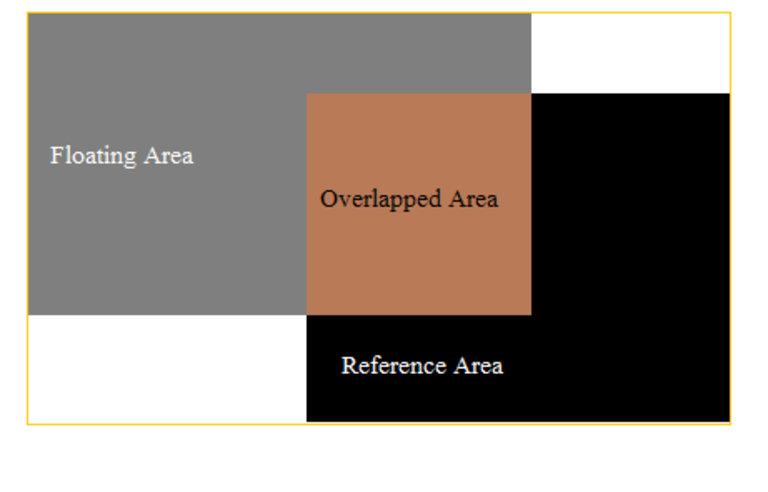
\includegraphics[width=\columnwidth]{2.mainmatter/2.Methodology/figures/Compositing}%
	\caption[Compositing]{Compositing of two images. The area within golden line is the compositing area. The gray area is floating image while black area is reference image.The overlapped area is painted with brown color.}%
	\label{fig:compositing-area}%
\end{figure}

\end{enumerate}

\item [\emph{Overlapping area identification}]
After we calculate the composite area i.e. the size of the stitched image, next task is to create an image with composite size and assign the pixel values of the float and reference images. Till now everything is okay except the overlapping areas. We assigned the overlapping pixels two times because those part is common to both floating and reference images (see figure~\ref{fig:compositing-area}). Since most of the real time problems, the overlapping areas are not same due to exposure differences and illumination which results visible seams in composite images. Again, we get blurred or ghosts in the overlapping region because of not accurate registration. To remedy these problem, we implement blending techniques. Some popular blending techniques are discussed in section~\ref{sec:blending}. Sometimes, if the intensity difference between images is large, the blending techniques are not capable of completely removing the visible seams~\cite{Dubrofsky:07}, we have to implement exposure compensation technique discussed in section~\ref{sec:exposure-compensation}.


\end{description}
\section{Blending}
\label{sec:blending}
The overlapping regions are blended for exposure compensation and mis-alignments. There are blending techniques which remove discontinuities in the composite image and create visually appealing stitched image. In this section, I am going to discuss some popular blending techniques: \emph{Optimal Seam Blending}, \emph{Alpha Blending} and \emph{Pyramid Blending}.
\subsection{Optimal Seam Blending}
\label{sec:optimal-seam-blending}
Optimal seam blending method search for a curve in the overlap region on which the difference of the images are minimal. If $I_1$ and $I_2$ are overlapping regions, for any y=$y_1$, a point (x,$y_1$) lies on the optimal seam curve if $I_1$(x,$y_1$) - $I_2$(x,$y_1$) is minimum for all x. Then, each image is copied to corresponding side of the seam. This simple method, however, does not give good result when there is global intensity difference between the images $I_1$ and $I_2$~\cite{levin:04}. 
\subsection{Alpha Blending}
\label{sec:alpha-blending}
Alpha blending, also called \emph{feathering}, is simple but effective algorithm. Alpha blending assigns the weight values (i.e. $\alpha$) to the pixels of the overlapping area. For $\alpha$=0.5, we get simple averaging, where both the overlapped areas will contribute equally to create stitched image. The value of $\alpha$ ranges from 0 to 1; if $\alpha$=0, then the pixel has no effect in composite region while $\alpha$=1 implies the pixel is copied there. Suppose, composite image $I$ is created from horizontally aligned images $I_1$ (left) and $I_2$ (right), then
\begin{equation}
I=\alpha I_1 + (1- \alpha)I_2
\label{eq:alpha-blending}
\end{equation}
Initially, we start with $\alpha$=1 (i.e. fully opaque) from $I_1$ until we reach overlap region. We go on decreasing $\alpha$ until it reaches to 0 (i.e. fully transparent) at the end of overlap region (see figure~\ref{fig:alpha-blending}).

\begin{figure}[H]%
\centering
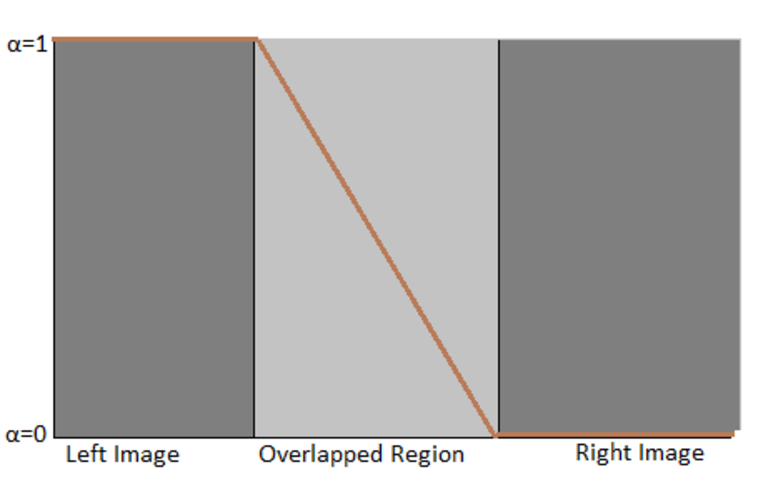
\includegraphics[width=0.9\columnwidth]{2.mainmatter/2.Methodology/figures/alpha-blending}%
\caption[Alpha Blending]{Alpha blending: $\alpha$ decreases from 1 to 0 in the overlapping region.}%
\label{fig:alpha-blending}%
\end{figure}

\noindent The above method is for horizontally aligned images; and similar technique can be used for vertically aligned images. If alignment is both horizontal and vertical, then left, right, top and bottom regions of the blending region will have effect in blending.\\

\noindent Alpha blending technique works well if the intensities of images $I_1$ and $I_2$ are similar. The advantage of alpha blending is its simplicity and we can tweak it to make it faster e.g. \emph{Look Up Table}~\cite{rankov:05}. 

%TODO The width of overlapped area effect in alpha blending
\subsection{Pyramid Blending}
\label{sec:laplacian-pyramid-blending}
The \emph{pyramid blending} uses image pyramids to blend and we use blending mask to mask the blended area. The blending mask assigns the weights of the pixels of the compositing images. The method consists of the following steps~\cite{Szeliski:06}:
\begin{itemize}
	\item Create Laplacian pyramids $L_1$ and $L_2$ from images $I_1$ and $I_2$.
	\item Create a Gaussian pyramid $G_M$ of the blending mask M. 
	\item Construct a combined pyramid $L_{combined}$ from $L_1$, $L_2$ and $G_M$ as:
	\begin{equation}
	L_{combined}(i,j)=G_M(i,j)*L_1(i,j)+(1-G_M(i,j))*L_2(i,j)
	\label{eq:combined_pyramid}
	\end{equation}
	\item Construct the blended image by collapsing the $L_{combined}$ pyramid.
\end{itemize}
The blending mask consists of the weights of the pixels in the compositing images $I_1$ and $I_2$. The values generally vary from 0 to 1 in the overlapping areas whereas either 0 or 1 in the non-overlapping parts. To make the process faster, the only overlapped areas are chosen for blending and other pixel are simply copied to the composite image.


\section{Exposure Compensation}
\label{sec:exposure-compensation}
The \emph{alpha blending} and \emph{pyramid blending} methods give a good blending result, compensate for moderate amounts of exposure difference between images. The methods, however, fail to give pleasing blending result when exposure difference become large~\cite{Szeliski:06}. This problem is more dominant if there is some rotation between the images while registration.\footnote{the rotated image will create extra pixels around the image which increases the complexity of the blending task.}\\

\noindent The transfer function based approach defined by Uyttendaele \emph{et al}~\cite{uyttendaele:01} seems to be effective to remove the exposure related artifacts. This method fits the block-based quadratic transfer function between each source image and an initial composite image. Then, the averaging of the transfer functions is carried out for smoother result. Per pixel transfer functions are calculated by interpolating between neighboring block values. This method does a better job of exposure compensation than simple feathering~\cite{uyttendaele:01}.\\

\noindent The above method can be simplified and faster by estimating the transfer function between the overlapped areas (i.e. $I_1$ $\Rightarrow$ $I_2$). Considering each and every pixels in the image makes the algorithm slower, so we only take care of true matching points. The transfer function parameters are estimated using a number of matched pairs\footnote{number depends upon the transfer function parameters e.g. linear transfer function $y=ax+b$, there are two unknown parameters to estimate, so we need two matched pairs}. The estimated transfer function maps the intensity of $I_1$ to intensity of $I_2$; thus works as an \emph{intensity leveling function}. 

\newpage
\section{Experimental Results}
This section presents some analysis and evaluation of blending algorithms with experimental data. The good blending algorithm should give visually appealing composite image with less change of image information and it should be computationally inexpensive. In the first part of experiment will select the best method among \emph{alpha blending} and \emph{pyramid blending}; and second part of experiment will focus on the tweaking of the selected algorithm to get the best optimized blended result for all alignments. 

\subsection{Alpha Blending versus Pyramid Blending}
In this section, I will present performance measures in terms of computational time and accuracy. The algorithms are implemented for both similar intensity and different intensity images. I have measured the time to produce the blended result for both the algorithms. The accuracy measurement is carried out in terms of error in pixel intensities from the corresponding actual pixels. 


\begin{table}[H]%
\centering
\begin{tabular}{|l|c|c|c|c|}
\hline
\multirow{3}{*}{Blending Method} & \multicolumn{2}{|c|}{Similar Intensity} & \multicolumn{2}{|c|}{Different Intensity}\\ \cline{2-5}
&Computational& Error & Computational& Error\\ 
& Time (seconds) &&Time (seconds)&\\\hline
Pyramid Blending&0.105 & 1278.8044&0.106 &18750.8828 \\ 
(Level2)&&&&\\ \hline
Pyramid Blending&0.119 &4097.8959 &0.140 &21644.5312 \\
(Level 4)&&&&\\ \hline
Alpha Blending & 0.015 & 260.5863&0.015 &17564.5039 \\ \hline
\end{tabular}
\caption{Alpha Blending versus Pyramid Blending}
\label{table:alpha-vs-pyramid}
\end{table}

\noindent From the table~\ref{table:alpha-vs-pyramid}, pyramid blending(level 2 and level 4) is taking longer time as compared to alpha blending. The error measurement shows that pyramid blending is losing more image information than alpha blending (see figure~\ref{fig:alpha-vs-pyramid}). The blended X-ray image should preserve image information and alpha blending is showing a better result than pyramid blending.

\begin{figure}[H]%
\centering
\subfloat[]{\label{fig:raw-composite}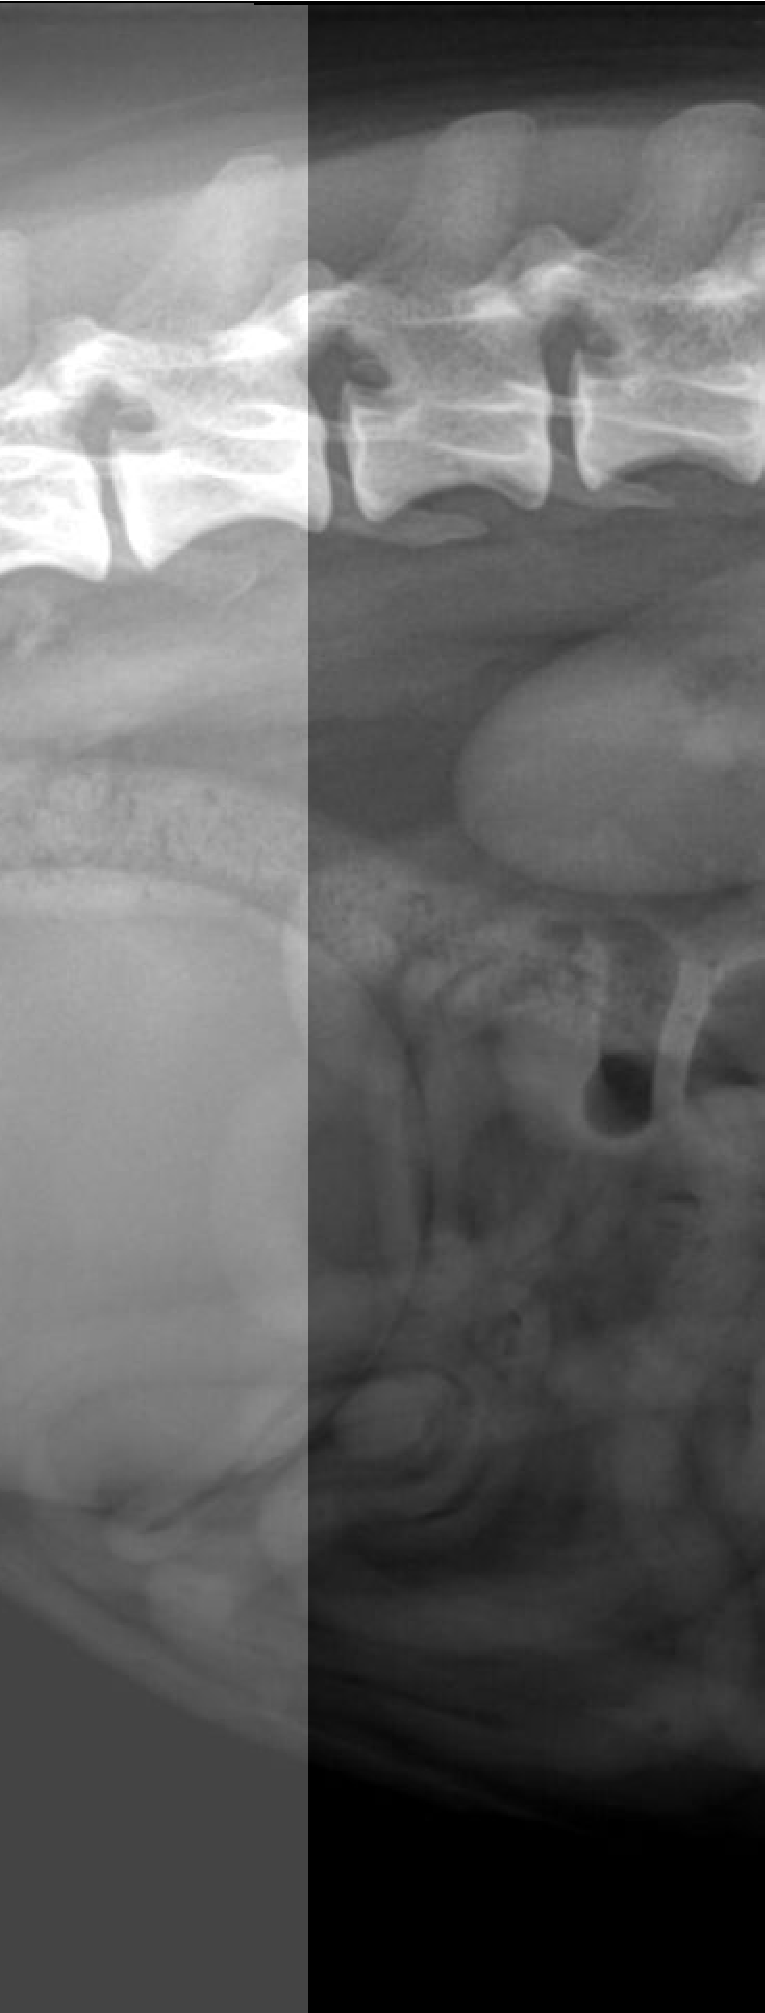
\includegraphics[scale=0.30]{2.mainmatter/2.Methodology/figures/raw-composite-image}} \quad
\subfloat[]{\label{fig:pyramid-4}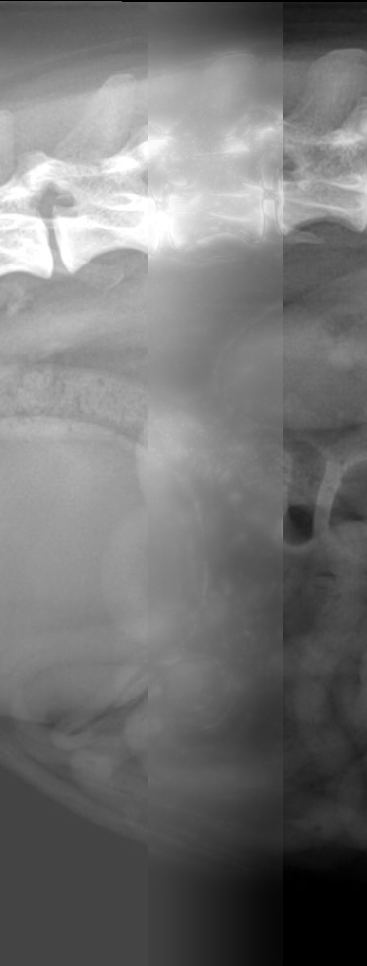
\includegraphics[scale=0.30]{2.mainmatter/2.Methodology/figures/stitched-image-pyramid-4}} \linebreak
\subfloat[]{\label{fig:pyramid-2}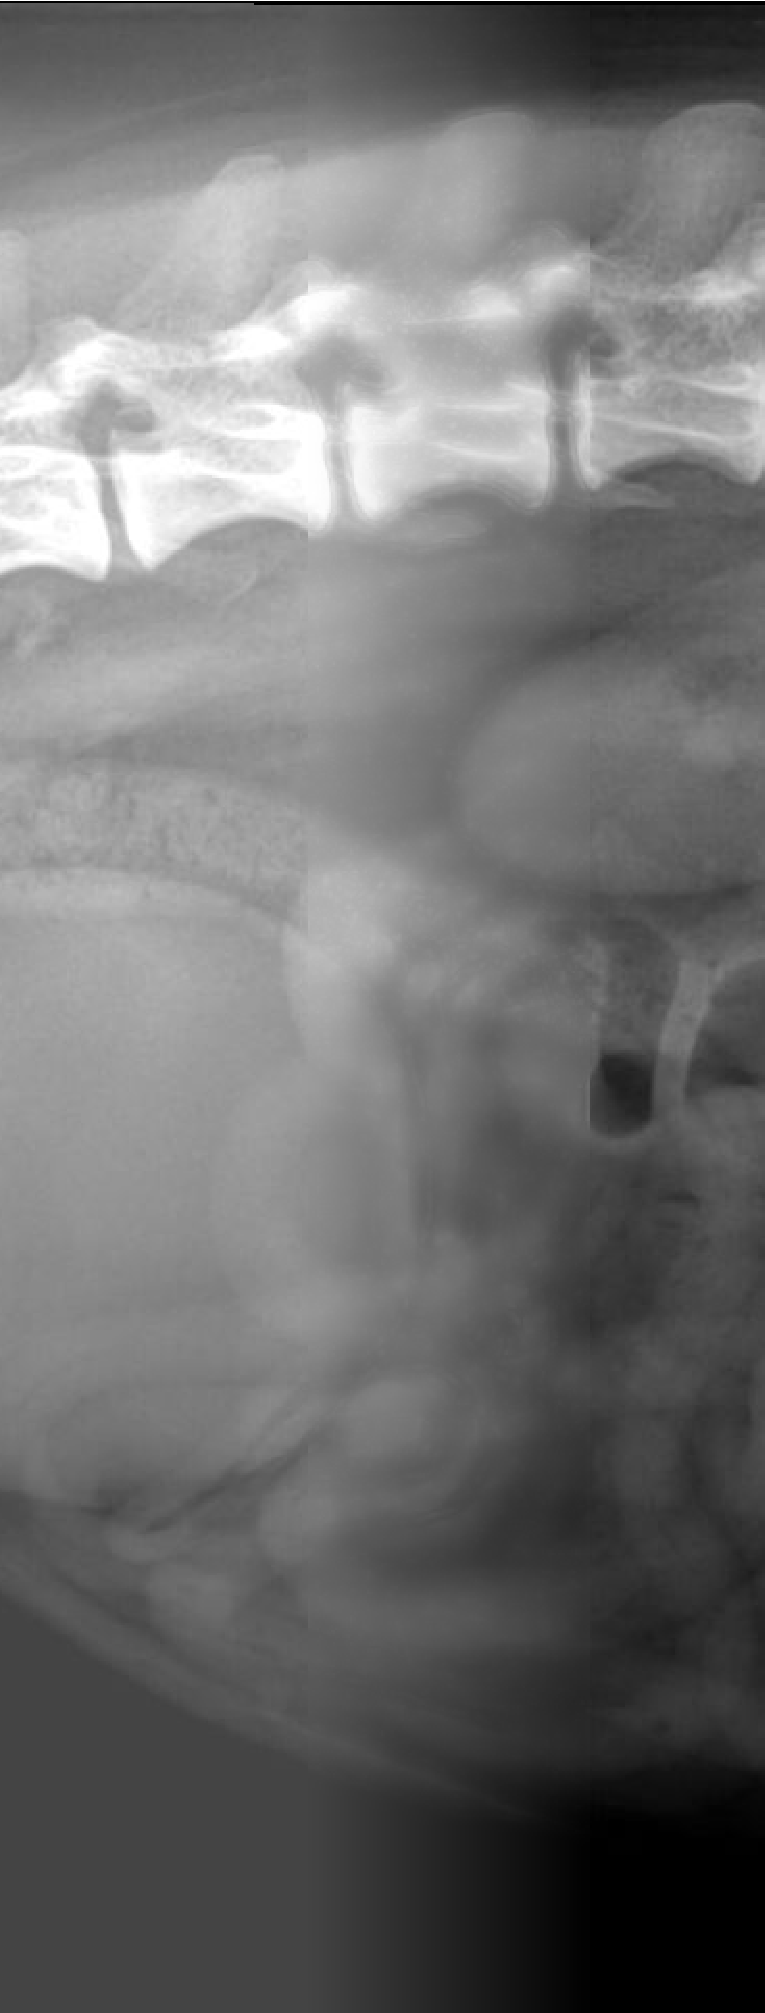
\includegraphics[scale=0.30]{2.mainmatter/2.Methodology/figures/stitched-image-pyramid-2}} \quad
\subfloat[]{\label{fig:alpha}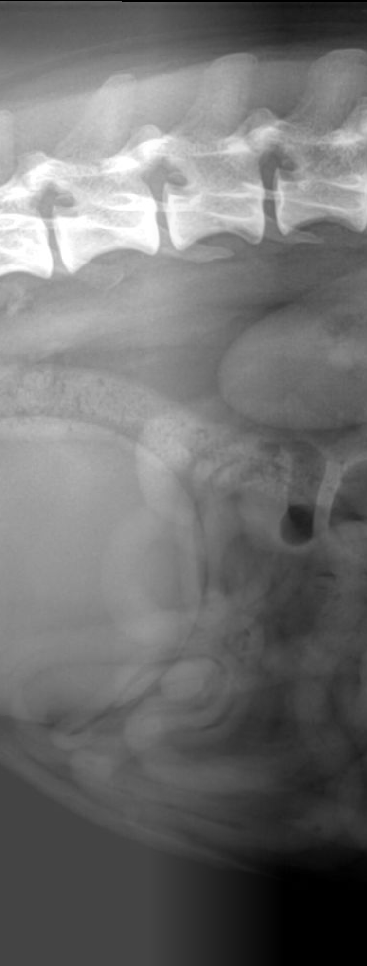
\includegraphics[scale=0.30]{2.mainmatter/2.Methodology/figures/stitched-image-alpha}}
\caption[Alpha Blending versus Pyramid Blending]{Comparison of results of Pyramid Blending and Alpha Blending. \subref{fig:raw-composite} is the composite image, \subref{fig:pyramid-4} is level 4 pyramid blended, \subref{fig:pyramid-2} is level 2 pyramid blended and \subref{fig:alpha} is alpha blended image. The blurring effect in Pyramid Blending is undesirable because it loses image information.}%
\label{fig:alpha-vs-pyramid}%
\end{figure}

\subsection{Blending Masks}
In the above section, I found alpha blending is faster and gives more accurate result as compared to pyramid blending. In this section, I will carry out experiments on the images with complex alignments. The horizontal or vertical blending for the image shown in figure~\ref{fig:multi-raw-composite-image} produces visible seams shown in figure~\ref{fig:single-alpha}.\\

\begin{figure}[H]%
\centering
\subfloat[]{\label{fig:multi-raw-composite-image} 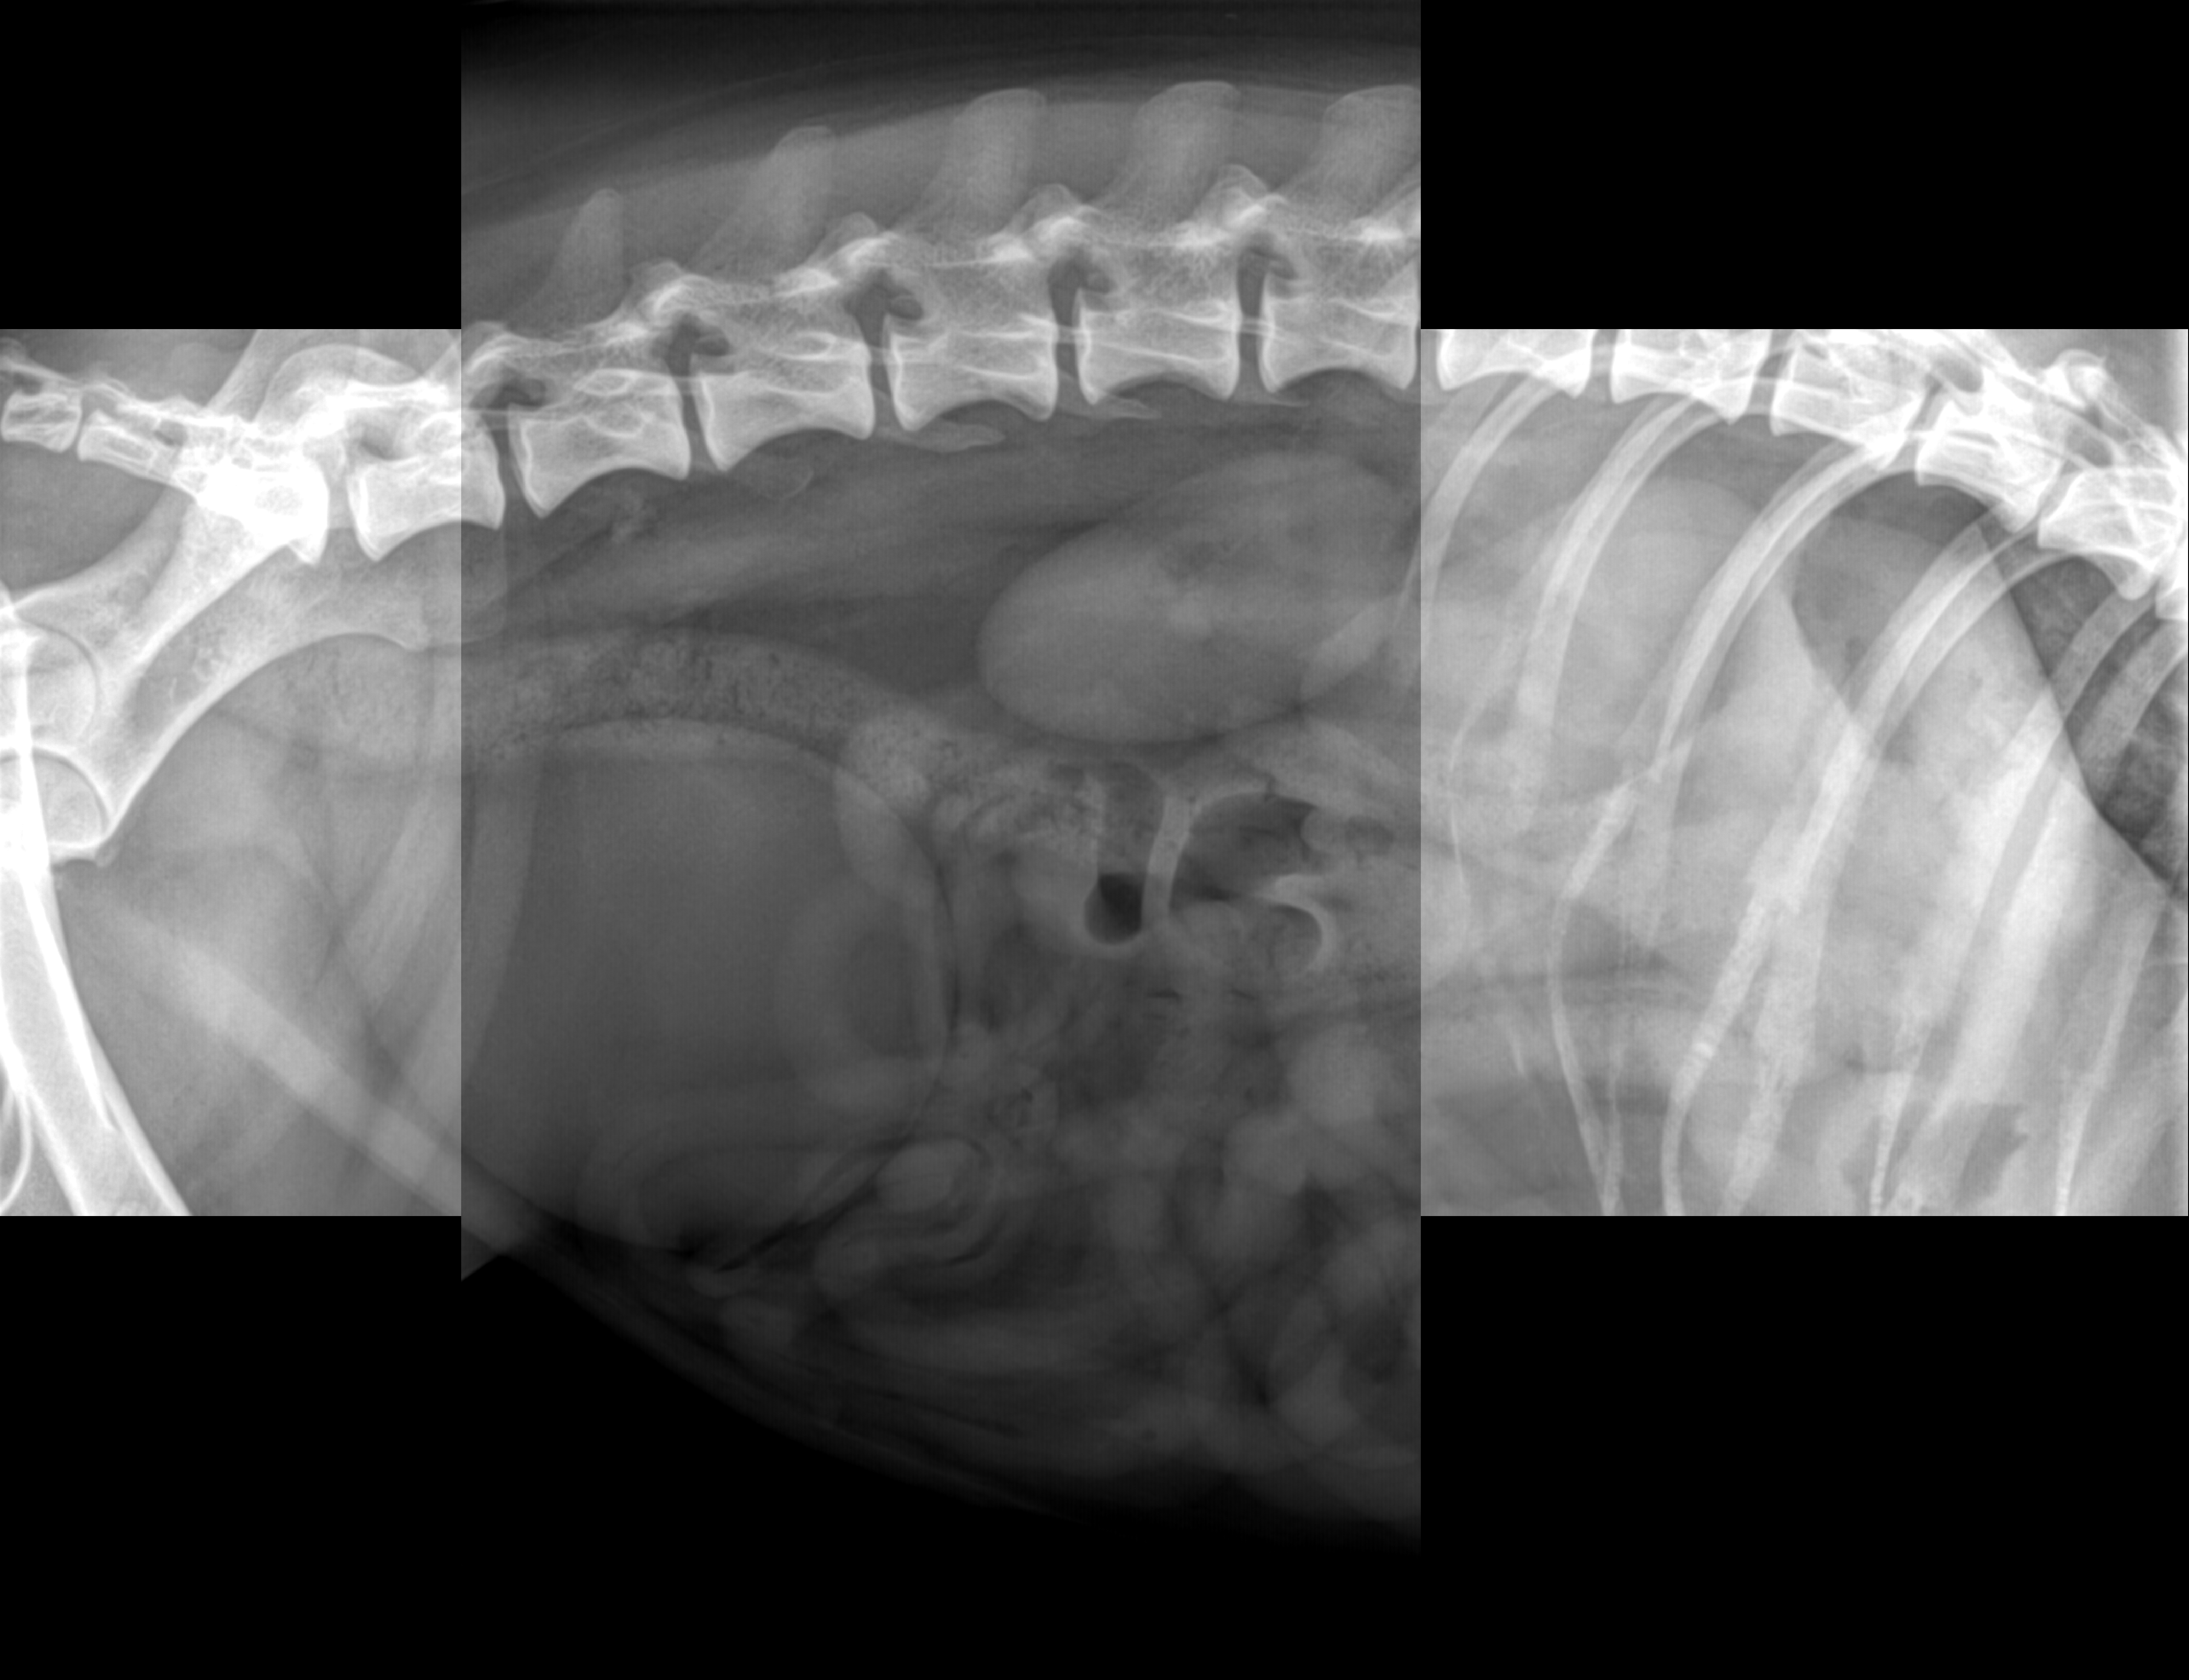
\includegraphics[scale=0.09]{2.mainmatter/2.Methodology/figures/multi-raw-composite-image}}
\subfloat[]{\label{fig:single-alpha} 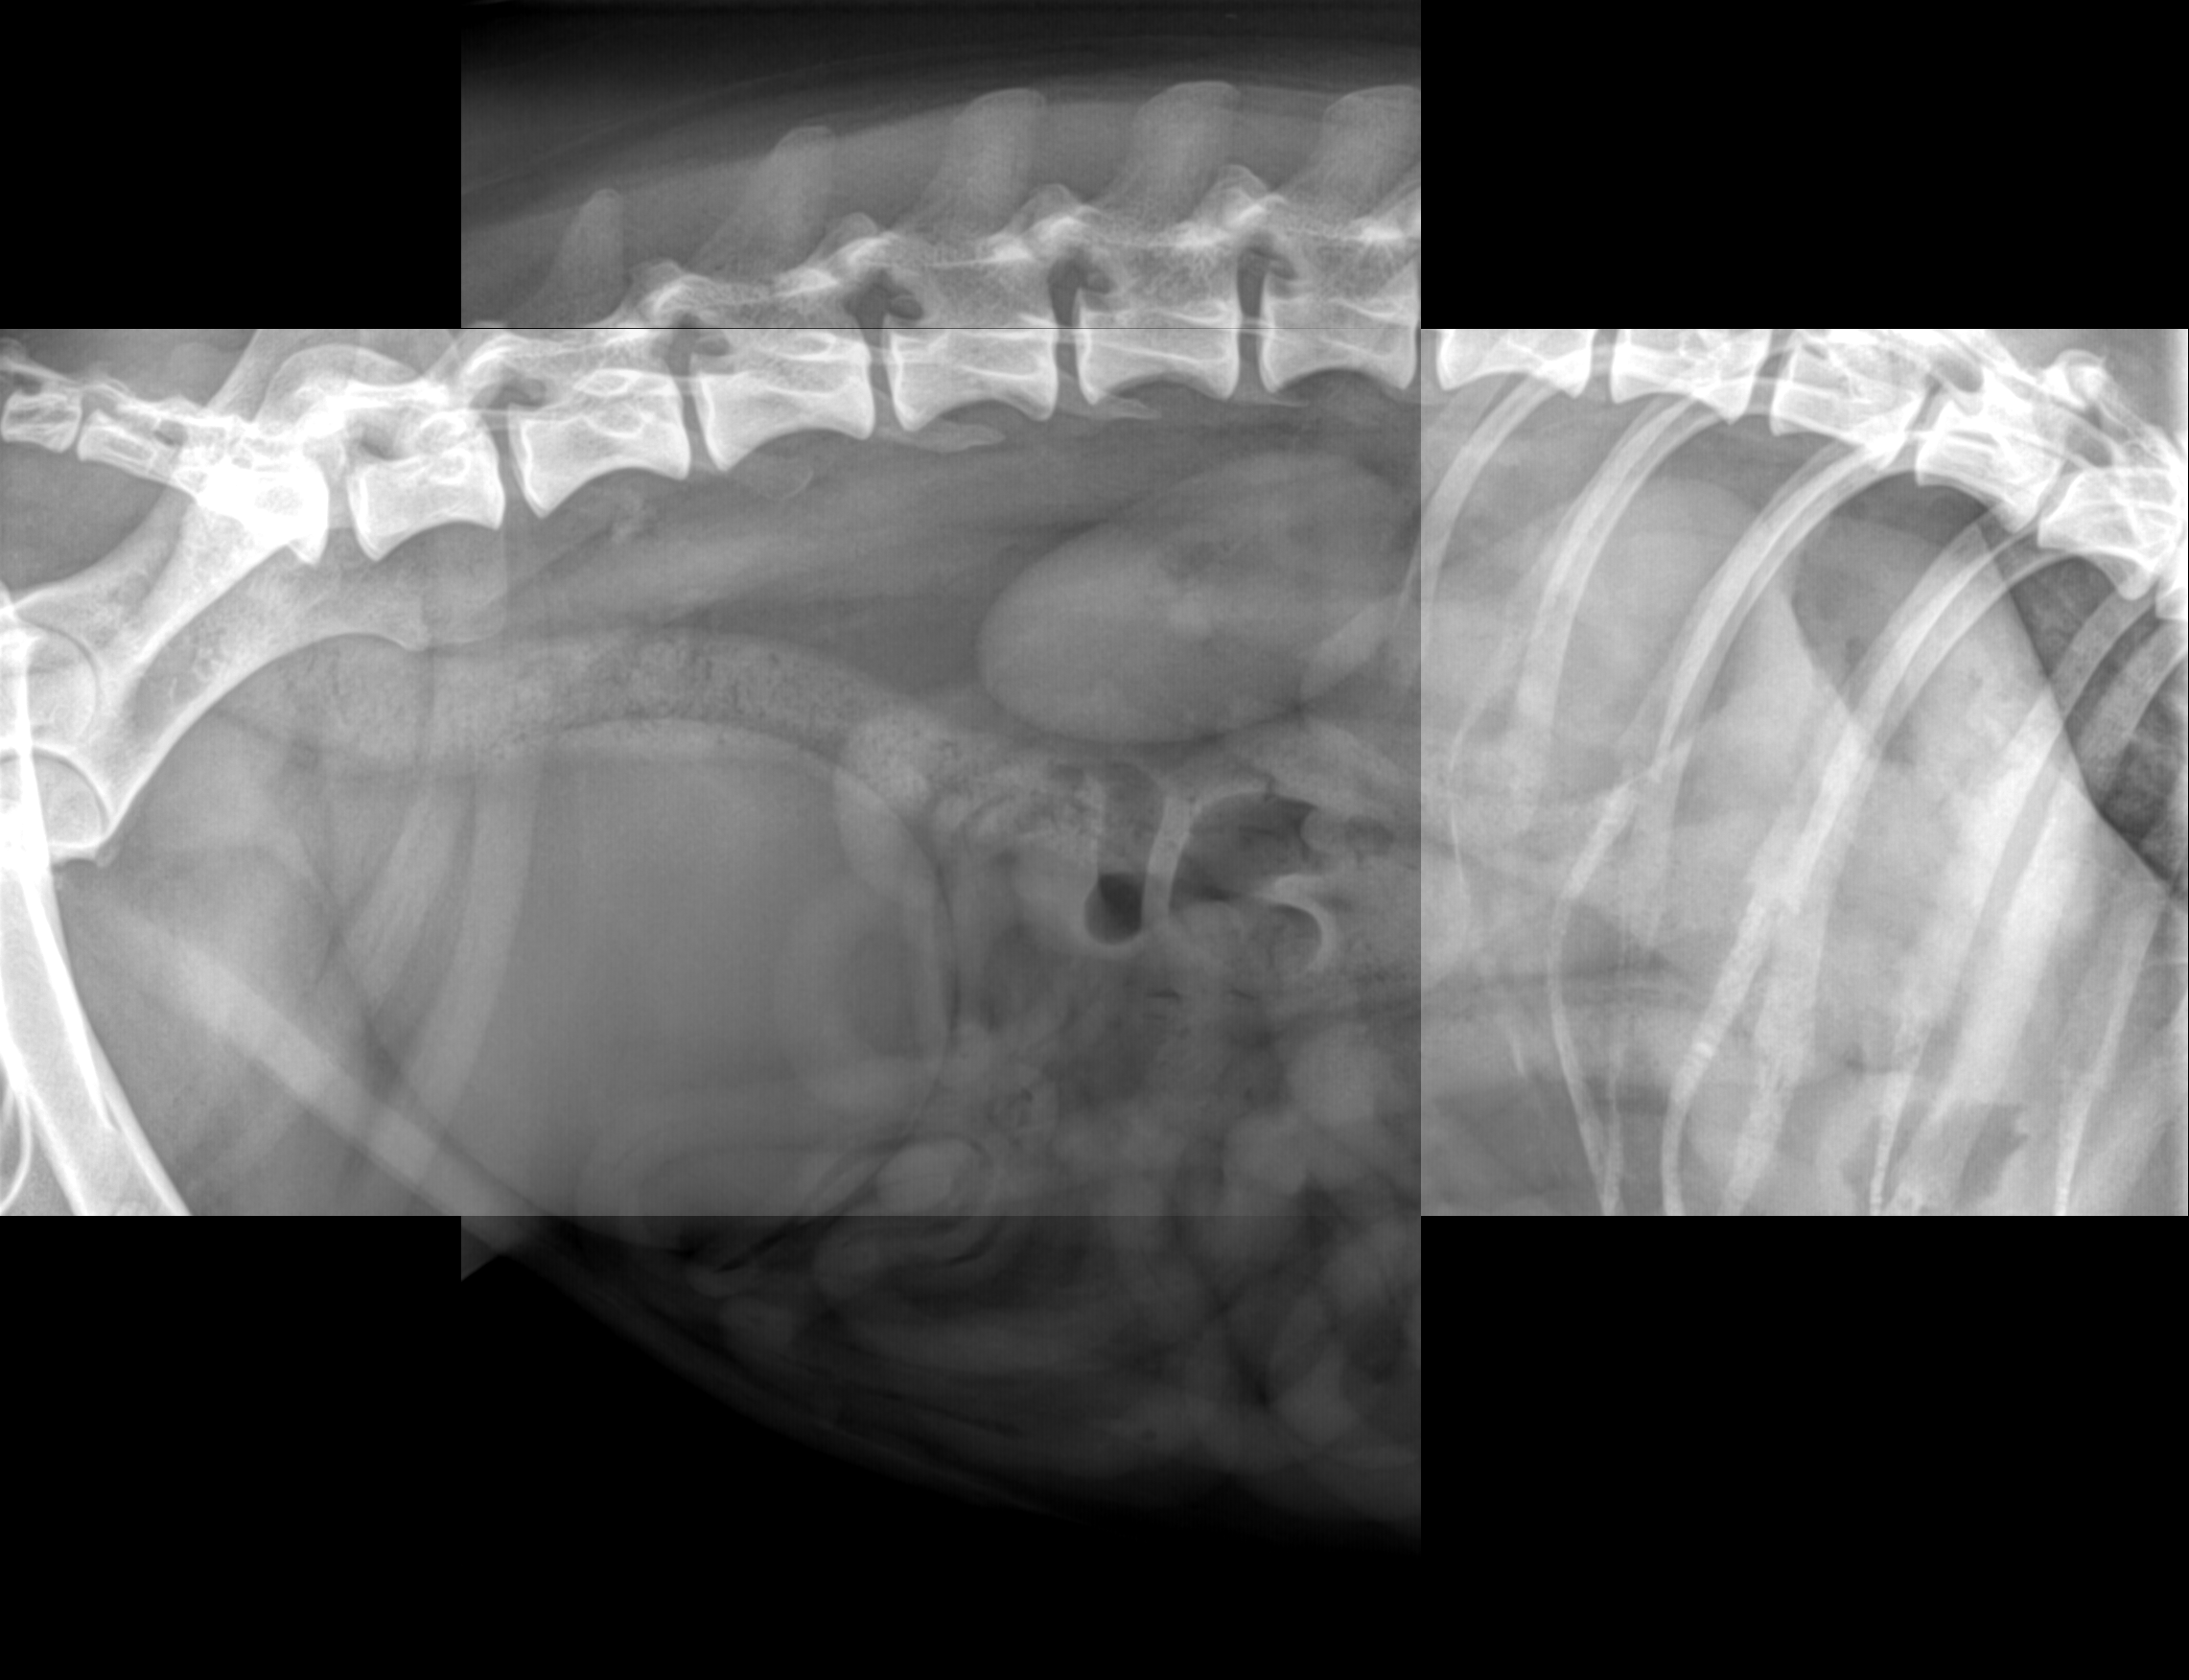
\includegraphics[scale=0.09]{2.mainmatter/2.Methodology/figures/single-alpha}}
\caption[Complex Alignment]{Figure \subref{fig:multi-raw-composite-image} is raw composite image, figure \subref{fig:single-alpha} is horizontally blended image. The seams are clearly visible on the join of the images.}%
\label{fig:blending-complex-alignment}%
\end{figure} 

\noindent So, to remedy this problem, a \emph{modified alpha blending method} has been implemented in which we create four blending masks (\emph{left}, \emph{top}, \emph{right}, \emph{bottom}) as shown in figure~\ref{fig:blending-masks}. The values in the mask indicates the effect of the image in the corresponding blending pixel (i.e. the higher value, the higher effect). For example, the left blending mask has higher values (shown white in the image) in left side means left image will have higher effect in the left side of the blended region to remove discontinuities in the composite image.\\


\begin{figure}[H]%
\centering
\subfloat[Left]{\label{fig:blending-mask1} 
\includegraphics[scale=0.1]{2.mainmatter/2.Methodology/figures/blending-mask-0}}
\subfloat[Top]{\label{fig:blending-mask2} 
\includegraphics[scale=0.1]{2.mainmatter/2.Methodology/figures/blending-mask-1}}
\subfloat[Right]{\label{fig:blending-mask3} 
\includegraphics[scale=0.1]{2.mainmatter/2.Methodology/figures/blending-mask-2}}
\subfloat[Bottom]{\label{fig:blending-mask4} 
\includegraphics[scale=0.1]{2.mainmatter/2.Methodology/figures/blending-mask-3}}
\caption[Blending Masks]{Blending masks. \subref{fig:blending-mask1} is mask for left image,\subref{fig:blending-mask2},\subref{fig:blending-mask3}, \subref{fig:blending-mask4} are masks for top, right and bottom images respectively.}
\label{fig:blending-masks}
\end{figure} 

\noindent The blended image using multiple blending masks is shown in figure~\ref{fig:blending-complex-alignment} which is far better than the image produced with either horizontal or vertical blending (compare images:~\ref{fig:single-alpha} and~\ref{fig:blending-complex-alignment})

\begin{figure}[H]%
\centering
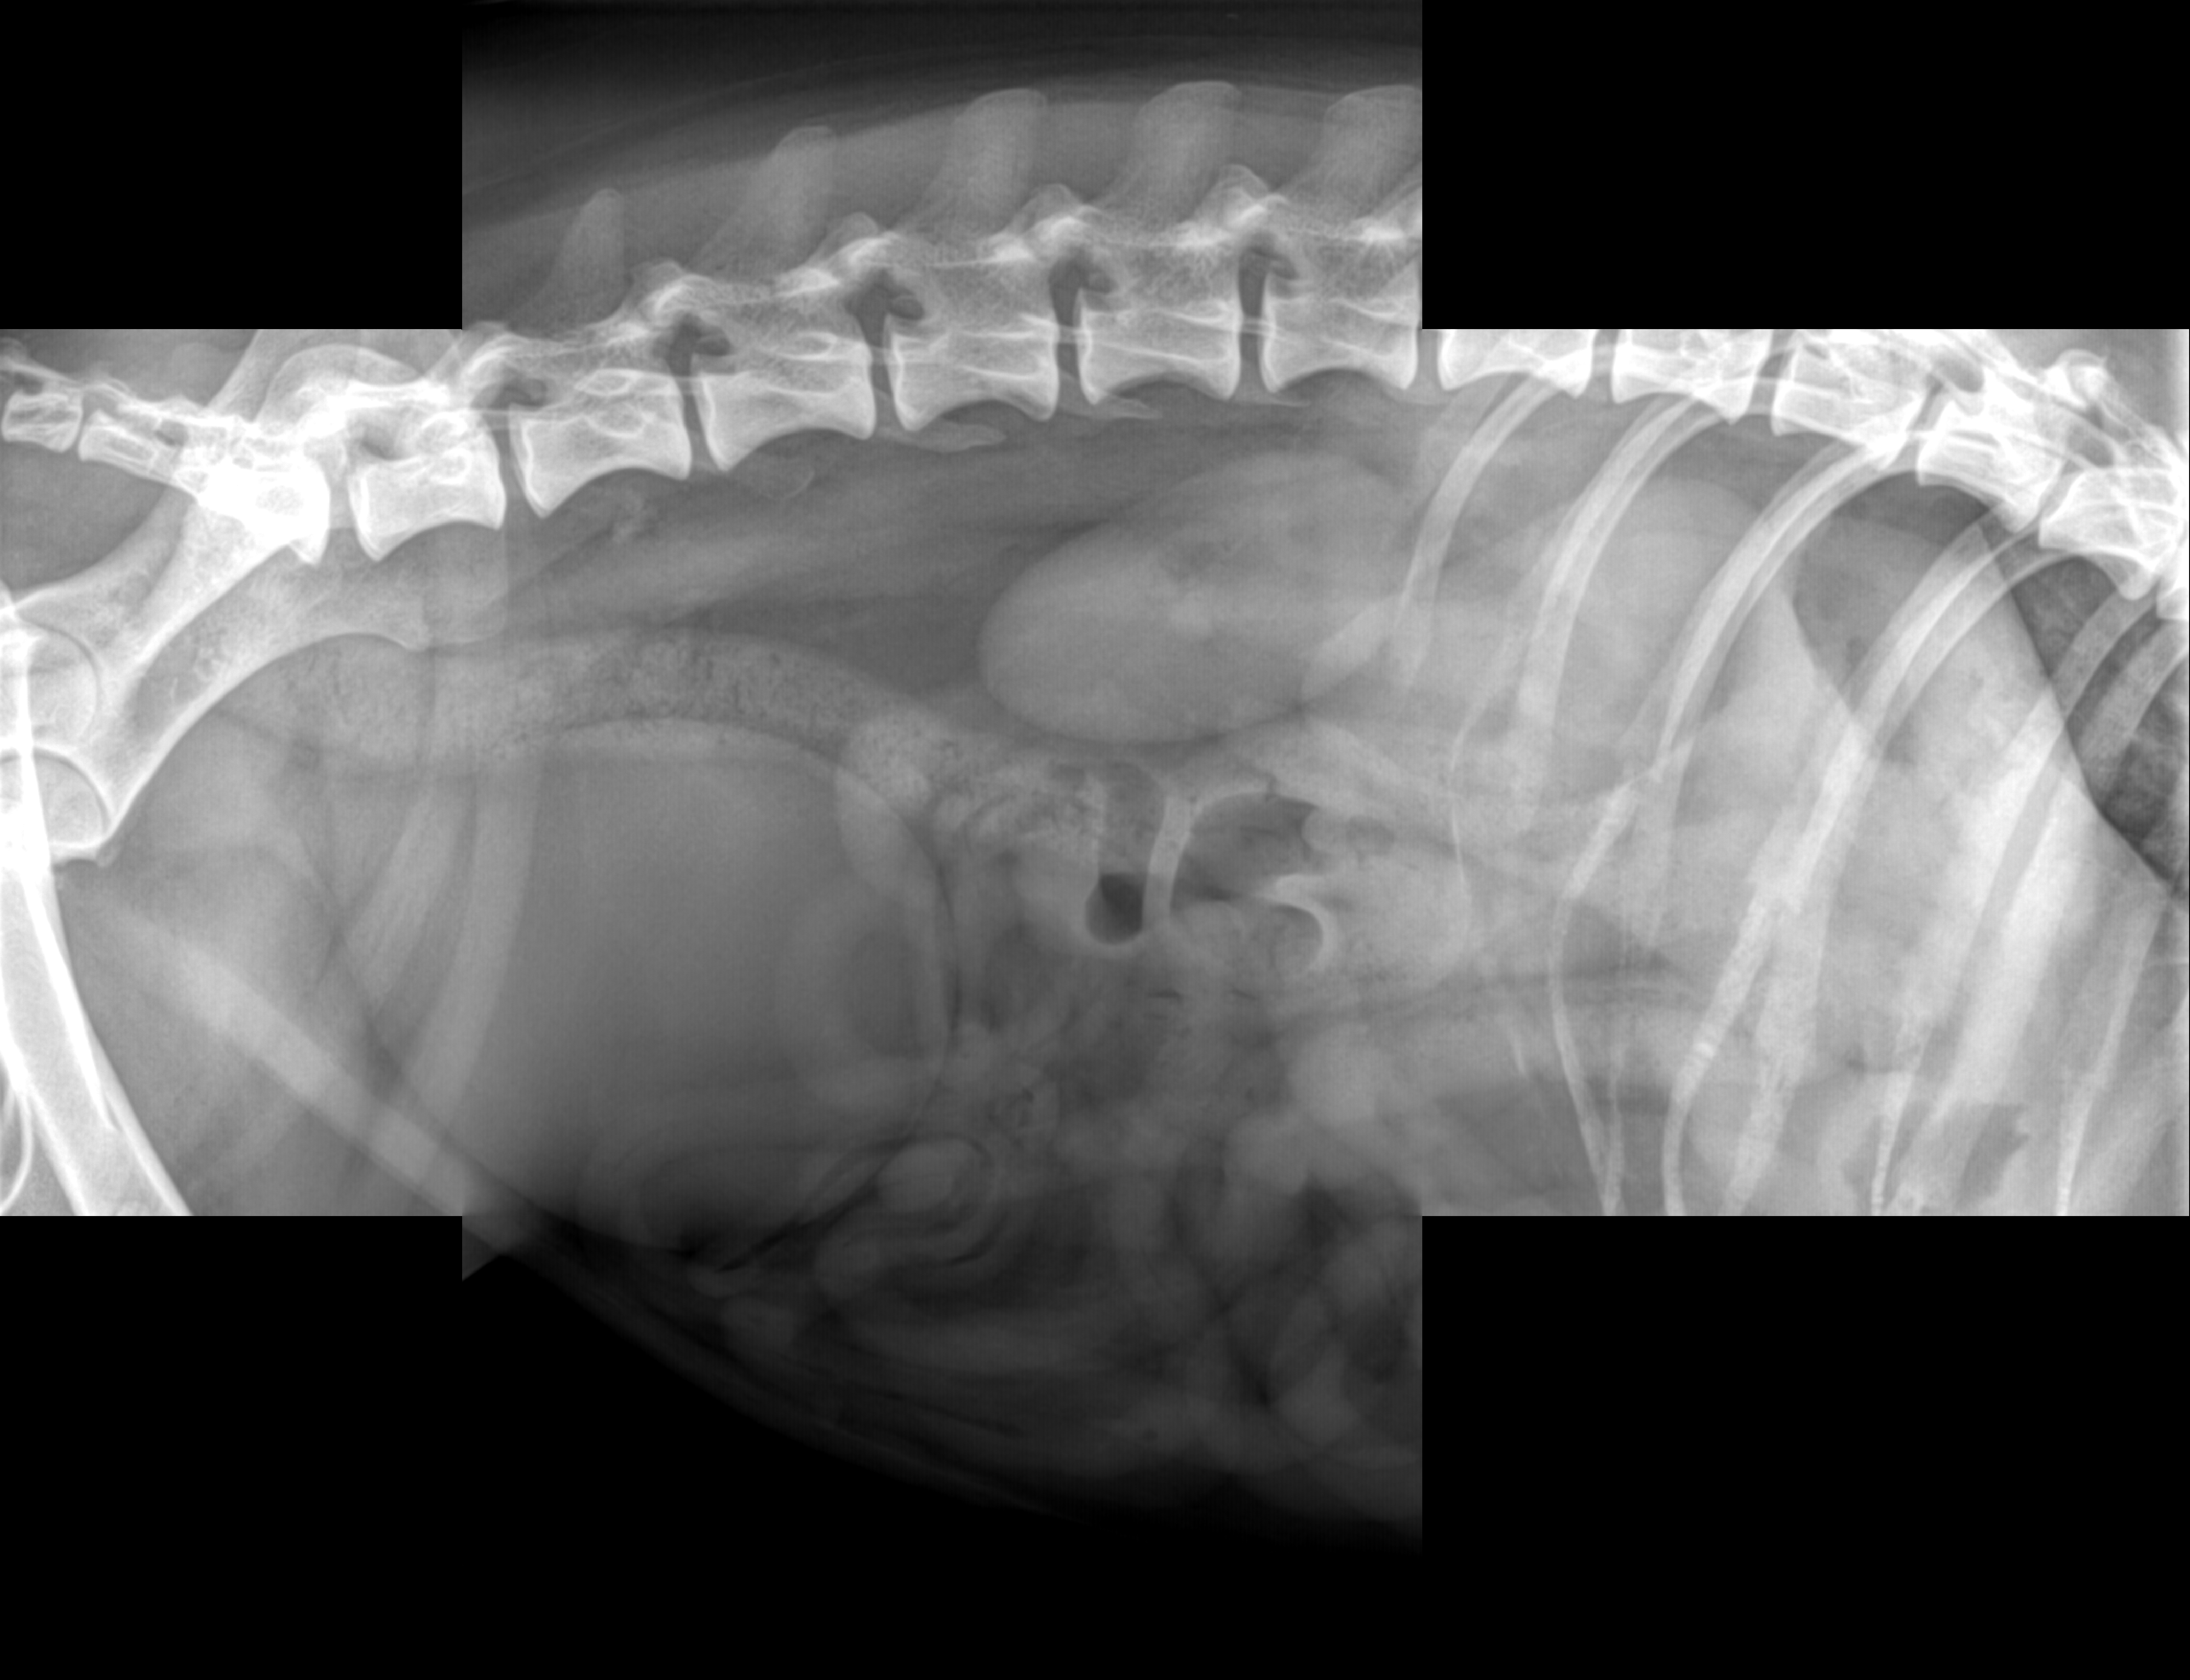
\includegraphics[scale=0.15]{2.mainmatter/2.Methodology/figures/multi-alpha}
\caption[Blending with Masks]{Use of multiple blending masks gives better blending result.}%
\label{fig:blending-complex-alignment}%
\end{figure}






